\input test/test
\input uvod/znacenie
\input uvod/uvod

\chapter{Fourierova transformácia}
    \input transformacia/historia
    \input transformacia/rady
    \input transformacia/gibbs
\section{Vlastnosti}
\section{Fourierova transformácia}
\section{Viacrozmerná fourierova transformácia}
\section{Príbuzní}

\chapter{Algoritmy}
    \section{Úvod}

Zopakujme si poznatky o diskrétnej Fourierovej transformácii.
\begin{definicia}
    Diskrétnou Fourierovou transformáciou postupnosti $x_0, \dots,
    x_{n-1}$ budeme označovať postupnosť $X_0, \dots, X_{n-1}$
    definovanú nasledovne
    \begin{equation}
        X_k = \sum_{l=0}^{n-1} x_l e^{-\frac{2\pi\imag}{n}kl}
        \label{eq:dft}
    \end{equation}
\label{def:dft}
\end{definicia}
Ak označíme \todo{roots of unity} ako
\begin{equation}
    \omega_{n,k} = e^ { -\frac{2\pi \imag}{n} k}
    \label{eq:omega}
\end{equation}
možeme predchádzajúcu definíciu prepísať na

\begin{equation}
    X_k = \sum_{l=0}^{n-1} x_l \omega_{n,k}^l =
          \sum_{l=0}^{n-1} x_l \omega_{n,kl}
    \label{eq:dft_omega}
\end{equation}

Pokračovať v tejto kapitole budeme najskôr najjednoduchšími
algoritmami pre počítanie fourierovej transformácie veľkosti mocnín
dvojky. Potom prejdeme na všeobecný prípad zložených čísel a následne
prvočísel. Kapitolu zavŕšime spomenutím ďalších algoritmov, o ktorých
existencii sa oplatí vedieť a ako čerešničku na torte pridáme
počítanie diskrétnej kosínovej transformácie.

    % vim:spell spelllang=sk
\section{DFT}

Začneme najzákladnejším algoritmom na výpočet diskrétnej Fourierovej
transformácie. Algoritmus vychádza priamo zo vzorca na výpočet
diskrétnej Fourierovej transformácie a uvedieme ho pre referenciu:

\begin{python}
class DFT:
    def transform(data):
        n = len(data)
        X = []
        for k in range(n):
            s = 0
            for l in range(n):
                s += data[l] * cmath.exp(- 2 * 1j * math.pi / n * k * l)
            X.append(s)
        return X
    transform = staticmethod(transform)
    
    def inverseTransform(data):
        n = len(data)
        X = []
        for k in range(n):
            s = 0
            for n in range(n):
                s += data[l] * cmath.exp(2 * 1j * math.pi / n * k * l)
            X.append(s / n)
        return X
    inverseTransform = staticmethod(inverseTransform)
\end{python}


    \section{decimation in time Radix2}

Pretým, než si ukážeme tento algoritmus, objavíme najskôr
krásu motýlích krídel\footnote{Z anglického názvu ``Butterfly''}.
To, čo robí štandardný DFT algoritmus pomalým, je jeho ignorancia.
Ignoruje totiž 2 veľmi dôležité fakty o komplexných koreňoch $\omega$,
ktorými sú
\begin{itemize}
 \item Symetria: $\omega_{n,k+n/2} = -\omega_{n,k}$, ak je $n$ párne
 \item Periodicita: $\omega_{n,k+n} = \omega_{n,k}$
\end{itemize}
Ich všímavým pozorovaním môžeme dospieť napríklad k nasledujúcemu
faktu:
\begin{equation}
\begin{split}
X_k & = \sum_{l=0}^{n-1} x_l \omega_{n,kl}, \qquad k=0,1,\dots,n-1 \\
    & = \sum_{l \rm{\:je\:párne}} x_l \omega_{n,kl}
      + \sum_{l \rm{\:je\:nepárne}} x_l \omega_{n,kl} \\
    & = \sum_{l=0}^{\lceil n/2 \rceil-1} x_{2l} \omega_{n,2kl} 
      + \sum_{l=0}^{\lfloor n/2 \rfloor-1} x_{2l+1} \omega_{n,k(2l+1)}
\end{split}
\end{equation}
V ďalšom texte budeme automaticky uvažovať prípad, že $n$ je párne.
Využijeme rovnosť $\omega_{n,k}^2 = \omega_{n/2,k}$ a výsledok upravíme na
tvar
\begin{equation}
\begin{split}
X_k & = \sum_{l=0}^{n/2-1} x_{2l} \omega_{n/2}^{kl} 
      + \omega_{n,k} \sum_{n=0}^{n/2-1} x_{2l+1} \omega_{n/2,kl}
\end{split}
\end{equation}
Nech $y_n=x_{2n}, \quad z_n=x_{2n+1}$. Potom $X_k = Y_k + \omega_{n,k}
Z_k$, kde $Y_k, Z_k$ sú $n/2$ bodové diskrétne Furierove transformácie
postupností $x$, resp. $y$ s periódou $n/2$, teda $Y_{n/2+k} = Y_k, Z_{n/2+k} = Z_k$.

Schématický výpočet $X_k, X_{n/2+k}$ z $Y_k, Z_k$ vidno na
nasledujúcom diagrame.
\todo{Butterfly}

K algoritmu už nie je dlhá cesta. Ak predpokladáme, že $n$ je mocnina
dvojky, vieme postupnosti $Y,Z$ vypočítať rekurzívne presne tým istým
algoritmom. Časová zložitosť algoritmu je $O(n\log n)$ ako sa môžeme
ľahko presvedčiť, nakoľko platí $T(n) = 2 T(n/2) + O(n)$.
Faktor o ktorom sme zatiaľ nehovorili je pamäť. Pri bežnom rekurzívnom
prístupe bude jej veľkosť taktiež $O(n \log n)$. Algoritmus sa ale
jednoducho dá zmeniť na "in-place" algoritmus, ktorý okrem vstupného
poľa bude potrebovať len konštantne veľa pamäti. Pozrime sa opäť na
výpočet algoritmu, tentokrát aj s rekurzívnymi volaniami.
\todo{obrazok}
Môžeme vidieť, že hodnoty $x_k$ sa používajú len v poslednom kroku
rekurzie, ich výstup sa používa len v predposlednom kroku rekurzie
atď. Algoritmus teda vieme prepísať jednoducho bez rekurzie.
Prvým krokom pred priamym výpočtom je je takzvané "bit reversal"
preusporiadanie. Je jednoduché zhliadnuť, že ak $k$ má binárny zápis
$b_m b_{m-1} \dots b_1 b_0$ kde $m = \log_2 n$, potom musíme
$x_k$ presunúť na pozíciu $b_0 b_1 \dots b_{m-1} b_m$. Jednoduchý
dôkaz tohoto tvrdenia: 
Predpokladajme, že chceme vypočítať $X_k, X_{n/2+k}$. Ak si povieme,
že použijeme (vypočítané) hodnoty $Y_k, Z_k$ a chceme aby zmena bola
na mieste, môžeme povedať, že $Y_k$ bude na mieste $X_k$ a $Z_k$ bude
na mieste $X_{n/2+k}$. Dáta pre $Y$ sa teda nachádzajú v prvoj
polovici poľa, zatiaľ čo dáta pre $Z$ v druhej polovici.
Keď si spomenieme, potrebné dáta na vypočítanie $Y$ sú práve tie $x_i$ kde $i$ je párne,
a dáta pre $Z$ tie, kde $i$ je nepárne. Teda, pred posledným krokom
musia byť najskôr všetky párne a potom všetky nepárne údaje. Keď sa
teraz pozrieme na výpočet $Y$ a $Z$, môžeme vidieť, že dáta v rámci
každej z týchto polovíc vstupu musia mať najskôr 2. bit nulový, a až
potom nasledujú údaje s 2. bitom nenulovým. Opakovaním tohoto postupu
nakoniec dôjdeme k spomínanému tvrdeniu o bitovom reverze.

    \section{Decimácia vo frekvencii radix2}
Toto je druhý bežne používaný algoritmus pre mocniny dvojky. Je veľmi
podobný decimácii v čase, ako si ukážeme. Avšak využíva iný rozklad
transformácie. Zamerajme sa tentoraz  špeciálne na výpočet párnych a
nepárnych indexov:
\begin{equation}
    \begin{split}
    X_{2k} &= \sum_{l=0}^{n-1} x_l \omega_{n,2kl} \\
            &= \sum_{l=0}^{n/2-1} x_l \omega_{n,2kl} +
              \sum_{l=0}^{n/2-1} x_{n/2+l} \omega_{n, 2k(n/2 + l)} \\
            &= \sum_{l=0}^{n/2-1} (x_l + x_{n/2+l}) \omega_{n, 2kl} \\
            &= \sum_{l=0}^{n/2-1} (x_l + x_{n/2+l}) \omega_{n/2, kl} 
    \end{split}
\end{equation}
Podobne, pre nepárne indexy platí
\begin{equation}
    \begin{split}
    X_{2k+1} &= \sum_{l=0}^{n-1} x_l \omega_{n,(2k+1)l} \\
            &= \sum_{l=0}^{n/2-1} x_l \omega_{n,(2k+1)l} +
              \sum_{l=0}^{n/2-1} x_{n/2+l} \omega_{n, (2k+1)(n/2 + l)} \\
            &= \sum_{l=0}^{n/2-1} (x_l - x_{n/2+l}) \omega_{n, (2k+1)l} \\
            &= \sum_{l=0}^{n/2-1} ((x_l - x_{n/2+l})
              \omega_{n,l} )
            \omega_{n/2, kl}
    \end{split}
\end{equation}
Posledné riadky predchádzajúcich rovníc sa podobajú na Fourierovu
transformáciu a môžeme ich na ňu prepísať:
\begin{align}
    X_{2k} &= DFT_{n/2}[x_l + x_{n/2+l}] \\
    X_{2k+1} &= DFT_{n/2}[(x_l - x_{n/2+l}) \omega_{n,l}]
\end{align}
Butterfly diagmam pre decimáciu vo frekvencii 
znázorňujúci práve vypočítaný fakt
vidíme na obrázku \ref{fig:butterfly_dif}

\begin{figure}[htp]
    \centering
        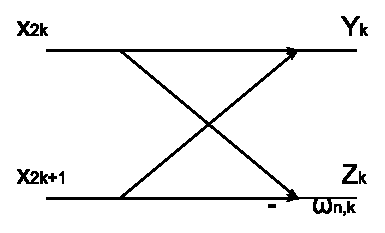
\includegraphics{obrazky/algoritmy/butterfly_dif}
        \caption{Butterfly diagram pre decimáciu vo frekvencii}
    \label{fig:butterfly_dif}
\end{figure}

Porovnaním s diagramom pre decimáciu v čase na obrázku
\ref{fig:butterfly_dit} môžeme
vidieť náramnú podobnosť. Vyzerá to tak, že butterfly pre decimáciu vo
frekvencii
je presne reverzným výpočtom butterfly pre decimáciu v čase. Toto
pozorovanie nie je náhodné, ako sa čitaťeľ môže presvedčiť. Dôsledok
je pozoruhodný - výpočet decimácie vo frekvencii 
prebieha presne v opačnom poradí
ako u decimácie v čase. Ilustrácia výpočtu pre $n=8$ sa dá nájsť na
ilustrácii \ref{fig:dif}

\begin{figure}[htp]
    \centering
        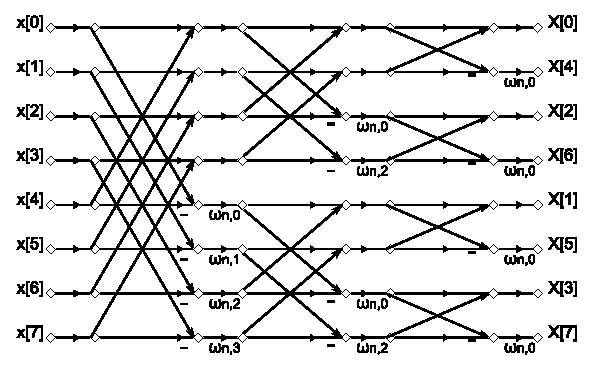
\includegraphics{obrazky/algoritmy/dif}
        \caption{Výpočet decimácie vo frekvencii pre $n=8$}
    \label{fig:dif}
\end{figure}
To, že výsledok je "bit reversed" nás neprekvapí a dôkaz je podobný
dôkazu u decimácie v čase.

\input code/dif
\todo{cite:dif}

    \section{Brunnov algoritmus}

Hoci je tento algoritmus nie veľmi používaný a menej numericky
stabilný ako doteraz popísané algoritmy, predsa ho len uvádzame.
Dôvod je jednoduchý - skrýva v sebe nápaditú a zaujímavú myšlienku,
ktorá si zaslúži pozornosť. Algoritmus využíva prístup založený na
polynómoch. Najskôr si však zhrnieme dôležité poznatky

\begin{lema}
    Pre polynón $x^k$ premennej $x$ a ľubovoľný konštantu $/alpha$
    platí
    \begin{equation}
        x^k \equiv \alpha^k \quad \mod x-\alpha
    \end{equation}
    kde $\mod$ je klasický zvyšok po delení polynómov
    \label{lema:polymod}
\end{lema}
\begin{dokaz}
    Spomeňme si na školský algebraický príklad
    \begin{equation}
        (x^k - y^k) = (x - y) (x^{k-1} + x^{k-2} y + \dots 
            + x y^{k-2} + y^{k-1})
    \end{equation}
    Potom zjavne
    \begin{equation}
        (x^k - \alpha^k) = (x - \alpha) * (\dots) \equiv 0 
        \quad mod x-\alpha
    \end{equation}
    čo ľahko upravíme na finálne tvrdenie
\end{dokaz}


Rovnicu \ref{eq:dft_omega} si
môžeme si ju predstaviť ako polynóm v premennej $\omega_{n,k}$.
Teda
\begin{equation}
    X(z) = \sum_{n=0}^{N-1} x_n z^n
\end{equation}
Kde za $z$ postupne dosadíme $\omega_{n,k}$ podľa
\ref{eq:omega}.
Podľa lemy \ref{lema:polymod} aplikovanej na súčet je vypočítanie
hodnoty polynómu v bode $t$ rovné zvyšku po delení $z-t$.
Celá úloha sa teda zmenila na $n$ počítaní zvyškov po delení polynómu
$X(z)$ polynómami $z-\omega_k, k=0,1,\dots,n-1$. Na prvý pohľad
rovnako ťažká úloha. Brunn sa ale nedal zastaviť a prišiel na
nasledujúci spôsob. Predpokladajme najskôr, že chceme počítať
diskrétnu Fourierovu transformáciu dĺžky ktorá je mocninou 2.
Existuje zovšeobecnenie aj pre iné zložené čísla, 
ktoré si uvedieme na konci kapitoly.
Základná myšlienka na ktorej budeme stavať je
\begin{lema}
    Nech $U,V$ sú polynómy. Potom pre všetky polynómy $X$ platí
    \begin{align}
        X \mod U &= (X \mod UV) \mod U \\
        X \mod V &= (X \mod UV) \mod V
    \end{align}
\end{lema}
\begin{dokaz}
    Dôkaz prenecháme ako jednoduché cvičenie čitateľovi.
\end{dokaz}
Nasleduje ďalšie pozorovanie, a to konkrétne
\begin{lema}
    $z^n - 1 = (z - \omega_0)(z-\omega_1)\dots(z-\omega_{n-1})$
\end{lema}
\begin{dokaz}
    $\forall k \in \{0,1,\dots,n-1\}: \omega_k$ je koreňom rovnice
    $z^n-1=0$ ako sa ľahko môžeme presvedčiť. Podľa základnej vety
    algebry, rovnica $n$-tého stupňa má najviac $n$ koreňov. Potom
    ale čísla $\omega_k$ musia byť nutne všetky korene $z^n-1$
    a teda $z^n-1$ sa dá zapísať tak ako bolo napísané.
\end{dokaz}
Celý Brunnov algoritmus je založený na šikovnej faktorizácii tohoto
polynómu. My si ho uvedieme pre mocniny dvojky, avšak existuje
všeobecnejšia verzia ktorá vie riešiť aj iné zložené čísla.
Všimnime si nasledujúcu lemu.
\begin{lema}
    \begin{align}
        z^{2k} -1 = (z^k - 1)( z^k + 1) \\
        z^{2k} + \alpha z^k + 1 = ( z^k + \beta z^{k/2} + 1)
            ( z^k - \beta z^{k/2} + 1), \quad
            \text{ pre }\alpha \in [-2,2], k\ge 2
    \end{align}
    kde $\beta = \sqrt{2-\alpha} \in [-2,2]$
\end{lema}
\begin{dokaz}
    Roznásobením pravých strán priamo dostávame pravé strany. V
    prípade druhej rovnice využívame navyše fakt $\alpha \in [-2,2]$
    aby sme mohli
\end{dokaz}
Jej pozoruhodnou vlastnosťou je, že ak vezmeme $n$ mocninu dvojky,
vieme $z^n-1$ postupne faktorizovať na polynómy polovičného stupňa,
každý s nanajvýš troma nenulovými členmi, a po $\log n$ fázach sa
dopracujeme na polynómy prvého stupňa, ktoré sú presne $z-\omega_k, 
k\in0,1,\dots,n-1$. 
Vráťme sa ale späť k algoritmu. Algoritmus začne vygenerovaním
polynómu $X(z)$. Následne vypočítame $X_{n,0} =X(z) \mod z^n -1$.
Pokračujeme $X_{n/2,0} = X_{n,0} \mod z^{n/2}-1$ a 
$X_{n/2,1} = X_{n,0} \mod z^{n/2}+1$. Je zjavné ako budeme pokračovať
ďalej, až dospejeme do stavu kedy sú polynómy kvadratické. Teraz nám
už nič nebráni vypočítať ich korene a pomocou lemy \ref{lema:polymod}
spočítať finálne výsledky $X_k, k\in 0,1,\dots,n-1$. Za pozornosť
stoja dve zmienky. Prvou je algoritmická zložitosť
$X_{2k,i} \mod z^{2k} + \alpha z^k + \beta$. Vďaka tomu, že polynóm,
ktorým delíme pozostáva len z troch členov, vieme ním deliť v
lineárnom čase od veľkosti prvého polynómu, teda v čase $O(k)$. V
$i$-tej fáze preto vykonáme $i$ delení o veľkosti $\frac{n}{2^i}$ a
$2i$ faktorizácii o konštantnom čase. Spolu teda lineárny čas pre
jednu fázu, fáz je $\log n$ a teda algoritmus má časovú
zložitosť $O(n \log n)$.
Druhom zmienkou je vec, ktorú sme doposiaľ zamlčali. Síce máme
vypočítané všetky hodnoty $X_k$, ale nevieme v akom poradí.
V tom sa nám hodí nasledujúca lema, pomocou ktorej vieme v každom
ktoku rekurzie preusporiadať hodnoty tak aby sme na konci dostali
$X_0,X_1,\dots,X_{n-1}$.
\begin{lema}
Nech $n\ge4$ je mocnina dvojky.
\begin{itemize}
\item
    Nech $x_0,\dots,x_{n/2}$ sú korene $z^{n/2} -1$ a
    $y_0,\dots,y_{n/2}$ sú korene $z_{n/2}+1$. Navyše, nech sú
    postupnosti $x_i, y_i$ usporiadané vzostupne podľa \todo{uhla}.
    Potom korene rovnice $z^n -1$ usporiadané podľa \todo{uhla} sú
    $x_0,y_0,x_1,y_1,\dots,x_{n-1},y_{n-1}$.
\item
    Podobne nech
    $x_0,\dots,x_{n/2}$ sú korene $z^{n/2} -\beta z^{n/4} +1$ a
    $y_0,\dots,y_{n/2}$ sú korene $z_{n/2} +\beta z^{n/4} +1$. Ako v
    predchádzajúcom prípade, nech sú
    postupnosti $x_i, y_i$ usporiadané vzostupne podľa \todo{uhla}.
    Potom korene rovnice $z^n +\alpha +1$ kde $\alpha,\beta$ sú v
    \todo{relacii ako v ref + todo a predpokladame ze alpha je
    dosiahnutelna rozkladom!!!} usporiadané podľa \todo{uhla} sú
    $x_0,y_0,y_1,x_1, \, x_2,y_2,y_3,x_3, \, \dots,
     x_{n/2-2},y_{n/2-2},y_{n/2-1},x_{n/2-1}$.

\end{itemize}
\end{lema}
\begin{dokaz}
Prvá časť dôkazu je jednoznačňe ľahšia. Môžeme sa ľahko presvedčiť, že korene
$z^{n/2}-1$ sú $\omega_{n,2i}$ a korene $z^{n/2}+1$ sú
$\omega_{n,2i+1}$ kde $i\in 0,1,\dots, n/2-1$. Navyše vieme, že spolu
tieto korene sú všetky korene polynómu $z^n-1$. Tvrdenie je potom
zjavné nakoľko uhol $\omega_{n,i}$ závisí lineárne od $i$.

Druhá časť dôkazu je väčší oriešok. Použijeme matematickú indukciu.
Predpokladajme na začiatku $n=4$.
Máme teda rovnicu
$z^4 + \alpha z^2 + 1 = (z^2 - \beta z + 1)(z^2 + \beta + 1)$.
Korene $x_0,x_1$ prvého polynómu pravej strany musia byť komplexne
združené, nakoľko predpokladáme $\beta\in[-2,2]$. To isté platí
aj o koreňoch $y_0,y_1$. Ak predpokladáme, že všetky 4 korene sú
rôzne, čo si môžeme dovoliť z predpokladu že daný polynóm vznikol
faktorizáciou $z^{n 2^m} -1$ pre nejaké $m\in\Nz$,
sú len 2 možnosti ich usporiadania -
buď $x_0,y_0,y_1,x_1$ alebo $y_0,x_0,x_1,y_1$ (Necháme na čitaťeľa si
premyslieť prečo). Stačí teda ukázať, že $\arg x_0 < \arg y_0$.
Jednoduchým výpočtom dostávame 
\begin{align}
    x = \frac{1}{2} (\beta \pm \sqrt{\beta^2 - 4})
    y = \frac{1}{2} (-\beta \pm \sqrt{\beta^2 - 4})
\end{align}
Nahliadnutím na štruktúru daných komplexných čísel a fakt $\beta\ge0$
ľahko vidíme, že $x$ má riešenie v prvom kvadrante zatiaľ čo $y$ až v
druhom. Tvrdenie pre $n=4$ sme dokázali.
Predpokladajme teraz, že tvrdenie platí pre nejaké $n\ge4$, ktoré je
mocninou dvojky.
Potom pre $2n$ platí nasledovné:
Korene $z^n - \beta z^{n/2} + 1$ sú $\sqrt{x_0},\sqrt{x_1},\sqrt{x_2},
\dots,\sqrt{x_{n/4-1}}$ a $ -\sqrt{x_0}, -\sqrt{x_1}, \dots,
-\sqrt{x_{n/4-1}}$. Navyše, vo vypísanom poradí sú aj zoradené podľa
uhla. Dôkaz je jednoduchý - odmocnením sme zmenili uhol u každého
koreňa na polovicu. Navyše platí $\arg -\sqrt{x}=\arg \sqrt{x} + \pi$.
Týmto je zabezpečená rastúcosť argumentu pre druhú polovicu koreňov.
A konečne, 
\begin{equation}
    \arg \sqrt{x_{n/4-1}} < \pi \le \arg -\sqrt{x_0}
    \label{eq:ineq_minus_sqrt}
\end{equation}
Podobný argument platí aj pre hodnoty $y$. Potom použitím indukčného
predpokladu na hodnoty 
$\sqrt{x_0},\dots \sqrt{x_{n/4-1}},
 \sqrt{y_0},\dots \sqrt{y_{n/4-1}}$ a
$-\sqrt{x_0},\dots -\sqrt{x_{n/4-1}},
 -\sqrt{y_0},\dots -\sqrt{y_{n/4-1}}$ plus
 využitím nerovnosti \ref{eq:ineq_minus_sqrt} dostávame požadované
 tvrdenie.
\end{dokaz}

Na záver bez dôkazu uvedieme rozklad polynómov pre všeobecný prípad.
\begin{veta}
\begin{equation}
    \Phi_{n,a}(z) = \left\{
        \begin{array}{l l}
            z^{2n} - 2\cos(2\pi a) z^n +1 & 0<a<1 \\
            z^{2n} -1 & 0=a
        \end{array}
    \right.
\end{equation}
Potom pre ľubovoľné $r\in\N$ také, že $r$ je deliteľom $n$ platí
\begin{equation}
    \Phi_{n,a}(z) = \left\{
    \begin{array}{l l}
        \Pi_{k=0}^{r-1} \Phi_{n/r, (a+k)/r} & 0<a\le 0.5 \\
        \Pi_{k=0}^{r-1} \Phi_{n/r, (1-a+k)/r} & 0.5<a<1 \\
        \Pi_{k=0}^{r-1} \Phi_{n/r, k/(2r)} & a=0

    \end{array}
    \right.
\end{equation}
\end{veta}

\todo{uhladit kod}
\input code/brunn

\todo{lit:http://www.economicexpert.com/a/Bruun:s:FFT:algorithm.htm}
\todo{lit:}
%http://en.wikipedia.org/wiki/Bruun's_FFT_algorithm

    \section{Cooley-Tukeyho algoritmus}
Tento algoritmus zobšeobecní predchádzajúce 2 algoritmy na
všeobecný prípad, keď je $n$ zložené. Jeho zaujímavou vlastnosťou je
tiež spojitosť fourierovej transformácie s jej dvojrozmernou verziou,
pretože toto je práve spôsob ako algoritmus funguje.
Nech $n=r_1 r_2$ kde $r_1,r_2>1$.
Zeveďme si
\begin{align}
    k &= k_1 r_1 + k_2, \quad &k_1 = 0,\dots,r_2-1, 
                \quad &k_2 = 0,\dots,r_1-1 \\
    l &= l_1  + l_2 r_2, \quad &l_1 = 0,\dots,r_2-1, 
                \quad &l_2 = 0,\dots,r_1-1 \\
\end{align}
Dané zobrazenie je bijekcia medzi $k \equivalence k_1,k_2$ a
$l \equivalence l_1,l_2$.
Pre zjednodušenie označenia si zaveďme $x_l = x_{l_1,l_2}$ a
$X_k = X_{k_1,k_2}$.

Potom rovnica \ref{eq:dft_omega} sa dá zapísať ako
\begin{equation}
    \begin{split}
    X_{k_1,k_2} = \sum_{l=0}^{n-1} x_l \omega_{n, (k_1 r_1 + k_2) l} \\
       = \sum_{l_1=0}^{r2-1} \sum_{l_2=0}^{r_1-1}
            x_{l_1,l_2} \omega_{n, (k_1 r_1 + k_2) (l_1 + l_2 r_2)}
    \end{split}
\end{equation}
Pretože $r_1 r_2 = n$, výraz v $\omega$ môžeme prepísať na
$\omega_{n, (k_1 r_1 + k_2) l_1} \omega_{n, k_2 l_2 r_2}$.
Zaveďme označenie $y$ nasledovne
\begin{equation}
    \begin{split}
    y_{l_1,k_2} = y_{l_1}[k_2] = 
        \sum_{l_2=0}^{r_1-1} x_{l_1,l_2} \omega_{n, k_2 l_2 r_2}  \\
       = \sum_{l_2=0}^{r_1-1} x_{l_1,l_2} \omega_{r_1, k_2 l_2}  \\        
        = DFT_{r_1}[x_{l_1}[l_2]]
    \end{split}
\end{equation}
kde sme explicitne zvýraznili indexy pre jednorozmernú Fourierovu
transformáciu, aby sa neplietli s fixnými indexami.
Potom 
\begin{equation}
    \begin{split}
    X_{k_1,k_2} = X[k_1]_{k_2}
     = \sum_{l_1=0}^{r_2-1} y_{l_1,k_2} \omega_{n,(k_1 r_1
    + k_2) l_1} =  \\
     \sum_{l_1=0}^{r_2-1}
     \omega_{n, k_2 l_1} \left( y[l_1]_{k_2} \omega_{r_2, k_1 l_1}
     \right)
    \end{split}
\end{equation}
Máme teda výraz pre DFT, až na twiddle faktory $\omega_{n,k_2 l_1}$,
pracovne nazvaný radix butterfly.
Cooley a Tukey vo svojej pôvodnej práci predpokladali, že na
vypočítanie tejto sumy je potrebný čas $O(r_2^2)$. 
Toto ale nie je pravda nakoľko radix butterfly sa dá tiež 
vypočítať pomocou DFT. Môžeme si všimnúť, že twiddle faktor závisí
len od $n, k_2$ čo sú v danom kroku konštanty a $l_1$. Preto môžeme
$y$ jednoducho vynásobiť twiddle faktorom a až potom počítať
transformáciu.

Nachvíľu sa teraz zastavme nad grafickou reprezentáciou algoritmu.
V prvom kroku si uložíme vstup $x$ do poľa veľkosti $r_2*r_1$ ($r_2$ riadkov a
$r_1$ stĺpcov), hodnoty ukladáme postupne po stĺpcoch.
Vstup pre $y_{l_1}[]$ je $x_{l_1,i}, i\in0,1,\dots,r_1-1$. Inak
povedané, $l_1$-tý riadok. Výstup môžeme uložiť do toho istého riadku.
Takto môžeme spracovať všetky riadky.
Následne hodnoty $y_{l_1, k_2}$ vynásobíme twiddle faktorom
$\omega_{n, k_2 l_1}$.
A teraz prichádza posledná fáza, kedy vstupom pre
 $X[]_{k_2}$ sú hodnoty $y[i]_{k_2}$, čiže $k_2$-ty stĺpec.
Cooley=Tukeyho algoritmus sa teda veľmi podobá na dvojrozmernú
Fourierovu transformáciu, jediný krok naviac je vynásobenie twiddle
faktormi v strede algoritmu.

Taktiež, Cooley-Tukeyho algoritmus je zobšeobecnením spomínaných
decimačných algoritmov - Decimácia v čase je Cooley-Tukeyho algoritmus
pre $r_1 =n/2, r_2=2$ (najskôr počíta transformácie polovičnej
veľkosti, následne spraví butterfly) a decimácia vo frekvencii je
$r_1=2, r_2=n/2$ (najskôr spraví butterfly a potom počíta
transformácie polovičnej veľkosti).

\begin{poznamka}
    Od tohoto okamihu budeme uvádzať iba programy, ktoré nie sú 
    "in place". Okrem iného to bude znamenať, že ich pamäťová
    zložitosť bude poväčšinou $O(n \log n)$. Toto neznamená, že dané
    programy sa nedajú prepísať aby boli "in place". V tejto horšej
    pamäťovej zložitosti ich budeme uvádzať z jednoduchého dôvodu -
    cieľom tejto publikácie je ukázať rôzne algoritmy, ich spojitosti
    a hlavné myšlienky. Uvádzaním in place algoritmov by sme preto len
    stratili na prehľadnosti a jednoduchosti programov.
\end{poznamka}
\input code/ct

\todo{lit:}
%http://en.wikipedia.org/wiki/Cooley-Tukey_FFT_algorithm
\todo{cite:cooley}

    % vim:spell spelllang=sk
\section{Bluesteinov algoritmus}

Už sme si ukázali rýchlu Fourierovu transformáciu na
mocninách dvojky a na zložených číslach. Čo nám ale stále
prekáža sú prvočísla, pre ktoré zatiľ nevieme rýchly algoritmus.
Jedným z algoritmov, ktorý pracuje na vstupe ľubovoľnej veľkosti
je práve Bluesteinov (tiež zvaný Chirp Z-transform) algoritmus.
Jeho výhodou je, že je všeobecnejší ako fourierova transformácia,
a to menovite vie rátať Z-transformácie.

\def\Ztransform{\mathcal{Z}}

\begin{definicia}[(Jednostranná) z-transformácia]
    Nech $x_n, n\in \Nz$ je postupnosť komplexných čísel a nech 
    $z\in\C$.
    Potom
    \begin{equation}
        X(z) = \Ztransform\{x[n]\} =
        \sum_{n=0}^{\infty} x_n z^{-n}
    \end{equation}
    Nazveme z-transformáciou postupnosti $x_n$.
\end{definicia}

Naším záujmom bude vypočítať z-transformáciu v $m$ po seme idúcich
bodoch.
Viac formálne, zaujíma nás výpočet
\begin{equation}
    X_k = \sum_{i=0}^{n-1} x_i z^{ik}, \quad k = 0,1,\dots,m-1
\end{equation}
\begin{poznamka}
    Je dobré si uvedomiť, že vypočítanie tej istej transformácie
    s $z_{\alpha + ik}$ je to isté ako násobenie výsledku
    $z_\alpha$ a teda vieme jednoducho riešiť aj tento všeobecnejší
    prípad.
\end{poznamka}

Celý algoritmus sa opiera o nasledujúci trik. Pre ľubovoľné čísla
$i,k$ platí identita
\begin{equation}
    ik = \frac{k^2}{2} + \frac{i^2}{2} - \frac{(i-k)^2}{2}
\end{equation}
Dosadením identity do rovnice a upravením dostávame
\begin{equation}
    X_k = z^{k^2/2}
        \sum_{i=0}^{n-1} 
            \left(x_i z^{i^2/2} \right)
            z^{-(i-k)^2/2}
        , \quad k = 0,1,\dots,m-1
\end{equation}
Na prvý pohľad sme nič nezjednodušili. To nie je celkom pravda,
pretože daná suma je konvolúcia. Presnejšie povedané nech
\begin{align}
    a_i &= x_i z^{i^2/2} \\
    b_i &= z^{-i^2/2} \\
    c_i &= z^{i^2/2}
\end{align}
Potom vieme danú sumu zapísať ako
\begin{equation}
    X_k = c_k \sum_{i=0}^{n-1} a_i b_{k-i}
\end{equation}
Zaťiaľ sme si veľmi nepomohli. Konvolúciu síce vieme spočítať pomocou
rýchlej Fourierovej transformácie, ale sme na mŕtvom bode, pretože
je opäť prvočíselnej veľkosti a navyše nie je cyklická. 
Tu ale prichádza k slovu hlavná pointa.
Konvolúciu nemusíme robiť o veľkosti $n$.
Presnejšie, nech $N\ge m+n -1$.
Rozšírme postupnosti $a_i,b_i$ nasledovne:
\begin{align}
    a_i &=0, \quad n\le i<N \\
    b_{N-i} &= b_{i}, \quad 0 < i < N \\
    b_i &= 0, \quad n\le i \le N-n
\end{align}
Potom
\begin{equation}
    X_k = c_k \sum_{i=0}^{N-1} a_i b_{k-i \mod N},
        \quad k = 0,1,\dots,m-1
\end{equation}
je cyklická konvolúcia, ktorú vieme počítať pomocou FFT.
Navyše, pokiaľ spĺňame podmienku $N\ge m+n-1$, $N$ môže byť ľubovoľné
číslo. Veľmi vhodnou voľbou je $N$ ako mocnina dvojky, v tomto prípade
$N < 2(m+n-1)$ a pomocou split-radix algoritmu vieme spraviť
konvolúcie v čase $O(N \log N)$.
Výsledok konvolúcie potom vieme upraviť v lineárnom čase na požadovaný
výstup. Preto časová zložitosť Bluesteinovho algoritmu je
$O( (m+n) \log (n+m))$.

\todo{uhladit kod}
\todo{vycisti tento kod - zaved staticke metody + vyuzi split-radix}
\begin{python}

import dct;
import cmath;

class Ztransform:
    def nextPowerOfTwo(self, x):
        i = 0
        x -= 1 # for power of two, we want same result
        while x > 0:
            i += 1
            x /= 2

        x = 1
        while i > 0:
            i -=1
            x *= 2
        return x
        
    def ztransform(self, data, z, m):
        n = len(data)
        N = self.nextPowerOfTwo(n+m-1)

        a = []
        b = []
        
        # prepare a
        for i in range(n):
            a.append(data[i] * z ** (0.5 * i * i))

        for i in range(N-n):
            a.append(0)

        # prepare b
        for i in range(0,m):
            b.append(z ** (-0.5 * i * i))

        for i in range(N-m-n):
            b.append(0)

        for i in range(n):
            k = n - i
            b.append(z ** (-0.5 * k * k))

        # do convolution
        tmp = dct.DFT();
        a = tmp.transform(a)
        b = tmp.transform(b);

        for i in range(N):
            a[i] *= b[i]

        a = tmp.inverseTransform(a)

        #prepare result
        result = []

        for i in range(m):
            result.append(a[i] * z ** (0.5 * i * i))

        return result

    def fft_transform(self, data):
        return self.ztransform(data, 
                               cmath.exp( -2* 1j* cmath.pi / len(data)),
                               len(data))

    def fft_inverse_transform(self, data):
        return self.ztransform(data, 
                               cmath.exp( 2* 1j* cmath.pi / len(data)),
                               len(data))

\end{python}


Bluesteinov algoritmus ako vidíme vie počítať Fourierovu transformáciu
pre prvočíselné dĺžky. Vie však toho viac. Jedným z jeho možných
použití je spektrálna analýza úzkeho pásu frekvencií.
Medzi ďalšie použitie platí napríklad analýza signálu s lineárne sa
meniaciou frekvenciou. Takéto signály sa vyskytujú pri fyzikálnom
pohybe vysielača a prijímača, ako sú napríklad satelity alebo analýza
signálov prichádzajúcich z vermíru. Viac o tomto použití sa dá dočítať
na konci
\cite{nasa}.


\todo{lit: http://www.economicexpert.com/a/Bluestein:s:FFT:algorithm.htm}
\todo{lit: http://en.wikipedia.org/wiki/Z-transform}
\todo{lit na dalsie studovanie + je tam aj rader a zrejme aj ine:}
%http://books.google.com/books?id=wzYuOF6HFX0C&pg=PA350&dq=bluestein+chirp+z+transform+algorithm&lr=&ei=D0u9Sf6mHJvuzQSQvei7Dw
\todo{lit o z transform:}
%http://books.google.com/books?id=SmDImt1zHXkC&pg=RA1-PA134&lpg=RA1-PA134&dq=chirp+z-transform+algorithm&source=bl&ots=5-xQ5-Zw9Q&sig=cI_bGlp6FJONbUvsrmv5ScvkLf4&hl=en&ei=mwm9SZupNIupsAbN_snZAw&sa=X&oi=book_result&resnum=5&ct=result


    \section{Raderov algoritmus}

    \section{Ďalšie algoritmy}

Algoritmov na výpočet rýchlej Fourierovej transformácie je nespočetne
veľa. Mnohé z týchto algoritmov sú len úpravami už spomínaných
algoritmov, snažiace sa poväčšinou o efektívnejšiu implementáciu -
využitie symetrie komplexných čísel, používanie reálnych čísel tam kde
treba a mnohé ďalšie optimalizácie až po efektívne ukladanie v pamäti
kvôli rýchlosti procesorovej cache. Ďalšie sú síce efektívne, ale v
dobe čoraz rýchlejších počítačov schopných paralelných výpočtov ich
algoritmická zložitosť prevažuje výhody, ako je to napríklad u
Winogradovho algoritmu. V tejto kapitole si spomenieme
niektoré ďalšie zaujímavé myšlienky, ale nebudeme ich rozoberať
podrobne, iba načrtneme výsledky.

\subsection{Split radix}

\subsection{Good-Thomas algorithm}

    \section{DCT}

Jednou z podobných transformácii k Fourierovej je diskrétna kosínová
transformácia, ktorú sme si uviedli v \todo{}. Ako uvidíme ďalej, táto
transformácia hrá dôležitú rolu v aplikáciach pri kompresii audia a
videa. Preto stojí za zmienku uistiť sa, že existuje efektívny
algoritmus na jej výpočet. V skutočnosti, väčšina algoritmov
popísaných v tejto práci sa dá s menšími či väčšími problémami
prerobiť na DCT. Preto si tieto algoritmy a ich úpravy nebudeme
uvádzať. To, čo si uvedieme je výpočet DCT priamo pomocou FFT s
predpracovaním údajov. Potom bude zrejmé, že DCT vieme počítať podobne
ako FFT (len s väčšou konštantou) v čase $O(n \log n)$,
čo bude pre nás postačujúce.
Začnime rovnicou pre DCT:
\begin{equation}
    X_k = \sum_{l=0}^{n-1} x_l \cos\left(
        \frac{\pi}{n} (l + \frac{1}{2}) k
        \right)
\end{equation}
ktorú upravíme do podoby
\begin{equation}
    X_k = \sum_{l=0}^{n-1} x_l \cos\left(
        \frac{\pi}{2n} (2l + 1) k
        \right)
\end{equation}

Pozrime sa teraz na Fourierovu transformáciu
\begin{equation}
    Y_p = \sum_{q=0}^{4n-1} y_q e^{-\frac{2\pi\imag}{4n} p q} =
          \sum_{q=0}^{4n-1} y_q \left(
                \cos ( \frac{\pi}{2 n} p q )
                + \imag \sin ( \frac{\pi}{2n} p q)
                \right)
\end{equation}
Našim cieľom je nájsť súvislosť medzi týmito dvoma zápismi. V prvom
rade, pri Fourierovej transformácii máme navyše imaginárnu časť,
ktorej by sme sa radi zbavili. Podobne ako vo Fourierových radoch
\todo{}, sínusové koeficienty vieme jednoducho vynulovať použitím
párnej symetrie. Presne povedané nech $y_q = y_{4n-q}, 0<q<4n$.
Potom
\begin{equation}
    Y_p =    \sum_{q=0}^{4n-1} y_q \left(
                \cos ( \frac{\pi}{2 n} p q )
                +  0 \imag 
                \right)
\end{equation}
Rovnice \todo{ref,ref} sa hneď viacej podobajú, stále ešte máme čo
upravovať. Vieme napríklad využiť symetriu kosínusu a upraviť $Y$ na
tvar

\begin{equation}
    Y_p =  y_{2n} \cos( \pi pq) - y_0 + 2 \sum_{q=0}^{2n-1} y_q 
                \cos ( \frac{\pi}{2 n} p q )
\end{equation}
Teraz je už ale jasné, kam vietor veje. Položme
\begin{align}
    y_{2l} &= 0, \quad & l\in 0,1, \dots, n-1
    y_{2l+1} &= x_l, \quad & l \in 0,1, \dots, n-1
\end{align}
Potom
\begin{equation}
    Y_p = 2 \sum_{l=0}^{n-1} y_l 
                \cos ( \frac{\pi}{2 n} p l ) = 2 X_p
\end{equation}
Diskrétnu kosínovú transformáciu teda vieme dostať ako
FFT vstupných dát, ktorým pridáme symetriu a na párne miesta vložíme
nuly.
\input code/dct_using_dft


\chapter{Použitie}
\section{Matematika}
    O matematickej časti Fourierovej transformácie sme hodne povedali hneď
v prvej kapitole. Jej veľkým prínosom bolo objavenie rozkladu funkcií
na ortonormálny systém, z ktorého analýza a algebra veľmi profitovali.
Preto sa touto myšlienkou nebudeme ďalej zaoberať. V tejto kapitole si
zhrnieme využitie Fourierových radov a transformácie hlavne na
riešenie parciálnych diferenciálnych rovníc a teda užitočnosť aj v
súčasnej dobe.

    \subsection{Separácia premenných}

Táto užitočná metóda na riešenie diferenciálnych rovníc uzrela prvý
krát svetlo sveta práve keď sa Fourier začal zaoberať riešením rovnice
tepla. Ukážeme si ju najskôr na jednorozmernom prípade vedenia tepla,
a následne na dvojrozmernom riešení Laplacovej rovnice obdĺžnikovej
oblasti.

\subsubsection{Rovnica vedenia tepla}

Uvažujme kovovú tyč. Aby sme si zjednodušili život, budeme používať
normalizované a teda bezrozmerné fyzikálne jednotky. Tyč bude mať
dĺžku 1 a bude tepelne izolovaná od okolia. Na začiatku bude mať
teplotu $T_0$ a jeden jej koniec ochladíme priložením na konštantnú
teplotu $T_1<T_0$. Formálne zapísané
$T(x,0) = T_0, 0<x\le1$ a $T(0,t)=T_1, 0\le t$. Druhý koniec je izolovaný a preto
cezeň nejde žiadny tepelný tok - podmienka ekvivalentná
$\pd{T}{x}(1,t)=0$. A finálne, posledná podmienka, podmienka
vedenia tepla, ako môže každý fyzik potvrdiť je
\begin{equation}
    \pd{T}{t} = \pdd{T}{x}, \quad0<x<1
    \label{eq:heat}
\end{equation}

Pojem separácie premenných je intuitívny. Začneme predpokladom
nezávislosti premenných. Presnejšie povedané, nech
$T(x,t) = X(x) F(t)$. Substituovaním do \ref{eq:heat}
dostávame
\begin{equation}
    \frac{X''}{X} = \frac{F'}{F} = - k^2
    \label{eq:separation}
\end{equation}
kde $-k^2$ je separačná konštanta. Znamienko mínus sme uhádli
fyzikálnou intuíciou - tyč sa bude postupne ochladzovať.
Pomôžeme si trochou analýzy:
\begin{lema}
    Rovnica $F'(t) = -k^2 F(t)$ má riešenie v tvare 
    $F(t) = C_0 e^{-k^2 t}$ kde $C_0 \in R$.
    Ďalej, rovnica $X'' + k^2 X = 0$ má riešenie v tvare
    $X(x) = C_0 \sin(k x) + C_1 \cos(k x)$. Navyše, tieto riešenia sú
    jediné riešenia danej rovnice.
\end{lema}
\begin{dokaz}
    Dôkaz je štandardnou súčasťou kurzu diferenciálnych rovníc a
    nebudeme ho uvádzať.
\end{dokaz}
Vyžitím tejto lemy a rovnice \ref{eq:separation} dostávame
\begin{equation}
    T(x,t) = (C_0 \sin (k x) + C_1 \cos (k x))(C_2 e^{-k^2 t})
\end{equation}
Okrajová podmienka $T(0,t) = 0$ a nenulovosť $e^{-k^2 t}$ 
implikuje $X(0)=0$ a teda $C_1 = 0$.
Podobne, podmienka nulového tepelného toku cez izolovaný koniec tyče
na druhom konci vedie k
$X'(1) = C_0 k \cos k = 0$. Každé nenulové riešenie potom musí spĺňať
\begin{equation}
    k = \frac{\pi}{2} + n \pi, \quad n \in \Z
\end{equation}
Výsledkom je teda spočítateľne veľa riešení $T$ v tvare $T=XF$,
menovite
$T_n = A_n \exp\left(-\pi^2 (n+\frac{1}{2})^2 t \right)
            \sin \left( \pi (n + \frac{1}{2}) x \right), n\in \Z$
Pretože daný problém je lineárny, každá lineárna kombinácia týchto
riešení musí byť riešením. Všeobecné riešenie je teda
\begin{equation}
T = \sum_{n=0}^{\infty} A_n \exp\left(-\pi^2 (n+\frac{1}{2})^2 t \right)
            \sin \left( \pi (n + \frac{1}{2}) x \right), n\in \Nz
    \label{eq:heat_expansion}
\end{equation}
kde sme využili fakt $\sin(-x) = -\sin(x)$ a teda sme s čistým
svedomím vynechali záporné indexy $n$.
Ostáva teraz jediná otázka, pravdupovediac tá najťažšia. Dá sa každé
riešenie \ref{eq:heat} zapísať ako \ref{eq:heat_expansion}. A v tomto
momente prichádzajú na rad Fourierove rady. Výsledok môžeme dosiahnuť
2 spôsobmi. Prvým je ručný výpočet
\begin{equation}
    \int_0^1 \sin\left(\pi(n+\frac{1}{2})x\right)
             \sin\left(\pi(m+\frac{1}{2})x\right) \dd x =
    \left\{
    \begin{array}{l l}
        0& m\not=n \\
        \frac{1}{2} & m=n
    \end{array}
    \right.
\end{equation}
a následná expanzia na otrogonálny systém. Poučnejšie pre čitateľa ale
bude nasledujúce odvodenie:

    \subsection{Výpočet $\pi$}

Vráťme sa k príkladu \todo{ref}.
Vieme, že
\begin{equation}
    S_n(x) = \frac{1}{2} + \frac{2}{\pi} 
        \sum_{m=1} \frac{\sin((2m-1)x}{2m-1}
\end{equation}
konverguje bodovo\footnote{spomeňme si na vetu \todo{ref}} 
k funkcii $f(x)=0, x\in (-\pi,0)$ a $f(x)=1, x\in (0,\pi)$.
To znamená, že čiastočné súčty konvergujú k hodnote $f(x)$ špeciálne
pre prípady $x=\frac{\pi}{4}$ a $x=\frac{\pi}{2}$. Dosadením do radu
dostávame
\begin{align}
   1= f(\frac{\pi}{4}) = \frac{1}{2} + \frac{2}{\pi}
    \sum_{m=1}^{\infty} \frac{\frac{\pi}{4} (2m-1)}{2m-1} \\
   1= f(\frac{\pi}{2}) = \frac{1}{2} + \frac{2}{\pi}
    \sum_{m=1}^{\infty} \frac{\frac{\pi}{2} (2m-1)}{2m-1} \\
\end{align}
resp.
\begin{align}
   \frac{1}{2}= \frac{2}{\pi}
    \sum_{m=1}^{\infty} \frac{\frac{\sqrt{2}}{2} (-1)^{\floor{m/2+1}}}{2m-1} \\
   \frac{1}{2} = \frac{2}{\pi}
    \sum_{m=1}^{\infty} \frac{(-1)^{2m-1}}{2m-1} \\
\end{align}
Prepísané do krajšej podoby
\begin{align}
    \frac{\pi}{4} = 1 - \frac{1}{3} + \frac{1}{5} - \frac{1}{7} +
    \frac{1}{9} - \frac{1}{11} + \cdots \\ 
    \frac{\pi}{2 \sqrt{2}} = 1 + \frac{1}{3} - \frac{1}{5} - \frac{1}{7} +
    \frac{1}{9} + \frac{1}{11} - \cdots \\
\end{align}

    \subsection{iseporimetric ineq.}

Fourierova transformácia má mnoho prekvapivých použití. Ako sme sa už
mohli presvedčiť, jej metódy sa dajú použiť na riešenie rôznych
problémov. Ako ďalšiu ukážku jej moci si dokážeme intuitívnu vetu.
Ešte predtým ale uvedieme jednu lemu:
\begin{lema}
  Nech $C$ je hladká uzavretá krivka na ploche. Potom ju možno popísať
  ako $(x(t),y(t))$ kde $t\in[-\pi,\pi]$ a $x(-\pi)=x(\pi),
  y(-\pi)=y(\pi)$ a navyše platí
  \begin{equation}
    \left(\frac{\dd x}{\dd t}\right)^2 +
    \left(\frac{\dd y}{\dd t}\right)^2 = konst.
  \end{equation}    
  \label{lema:ekvidist_parametric}
\end{lema}
\begin{dokaz}
    Krivka je hladká a môžeme ju parametricky popísať ako
    \begin{equation}
        \left(x(t),y(t)\right), \quad t\in[-\pi,\pi]
    \end{equation}
    kde $x,y$ sú spojité funkcie spĺňajúce $x(-\pi)=x(\pi), y(-\pi)=y(\pi)$.
  Označme
   \begin{equation}
        s(t) = \int_{-\pi}^t \sqrt{ (x'(w))^2 + (y'(w))^2} \dd w
   \end{equation}
   Môžeme si všimnúť, že $s(t)$ je rastúca a preto je monotónna
   (Funkcie $x'(w)$ a $y'(w)$ nemôžu byť obe nulové na spoločnom intervale,
   lebo by to bolo v spore s monotónnosťou parametrického popisu)-
   Zaveďme
    \begin{equation}
        \dual{t} = -\pi + \frac{2 \pi s(t)}{s(\pi)}
    \end{equation}
   Podľa pozorovania o monotónnosti, vieme že zobrazenie
   $t\imply \dual{t}$ je bijekcia a preto existujú (spojité funkcie)
   $\dual{x},\dual{y}$ spĺňajúce
   \begin{equation}
        (\dual{x}(\dual{t}),\dual{y}(\dual{t})) = (x(t),y(t))
   \end{equation}
   Potom
   \begin{equation}
        x'(t) = \dual{x}'(\dual{t}) =
        (\dual{x}(-\pi + \frac{2 \pi s(t)}{s(\pi)})' =
        \dual{x}'(-\pi + \frac{2 \pi s(t)}{s(\pi)} 
        \frac{2\pi}{s(\pi)}
        \sqrt{ (x'(t))^2 + (y'(t))^2)} =
        \dual{x}'(\dual{t}) \frac{2\pi}{s(\pi)}
        \sqrt{ (x'(t))^2 + (y'(t))^2)}
   \end{equation}
   a po troche úprav dostávame finálnu podobu   
   \begin{equation}
    \left(\frac{\dd \dual{x}}{\dd \dual{t}}\right)^2 +
    \left(\frac{\dd \dual{y}}{\dd \dual{t}}\right)^2 = 
    \frac{s(\pi)}{2\pi}^2
    \label{eq:ekvidist_parametric}
   \end{equation}
\end{dokaz}

\begin{veta}
Nech $C$ je hladká uzavretá krivka na ploche. Nech $S$ je jej obsah a $O$ je
jej obvod. Potom
    \begin{equation}
      4\pi S \le O^2
    \end{equation}
\end{veta}

\begin{dokaz}
    Podľa lemy \ref{lema:ekvidist_parametric} existujú
    $x(t),y(t), t\in[-\pi,\pi]$ spĺňajúce rovnicu
    \ref{eq:ekvidist_parametric}.
    Vzorce pre objem a obvod sa pomocou nich dajú vyjadriť ako
    \begin{align}        
        O =& \intpipi \sqrt{\left(\frac{\dd x}{\dd t} \right)^2 +
            \left(\frac{\dd y}{\dd t} \right)^2} \dd t = s(\pi) \\
        S =& \intpipi x \frac{\dd y}{\dd t} \dd t    
    \end{align}
    Pretože $x,y$ sú hladké \todo{niekde definovat hladkost}, môžeme
    ich podľa vety \todo{ref: rovnomerna konvergencia}
    zapísať ako
    \begin{align}
        x(t) &= \frac{a_0}{2} + \sum_{n=1}^{\infty} \left(
               a_n \cos(n t) + b_n \sin(n t) \right) \\
        y(t) &= \frac{c_0}{2} + \sum_{n=1}^{\infty} \left(
               c_n \cos(n t) + d_n \sin(n t) \right)
    \end{align}
    Podľa \todo{ref: derivacia radu} navyše platí
    \begin{align}
        x'(t) &= \sum_{n=1}^{\infty} n \left(
            -a_n \sin(nt) + b_n \cos(n t) \right) \\
        x'(t) &= \sum_{n=1}^{\infty} n \left(
            -c_n \sin(nt) + d_n \cos(n t) \right)
    \end{align}
    \todo{perseval} implikuje s použitím
    \todo{nasledujuca vec neplati}
    \begin{equation}
    \begin{split}
        \frac{O^2}{2\pi} &= \intpipi ((x')^2 + (y')^2) \dd t \\
        &=
        \intpipi \sum_{n=1}^{\infty} n^2 \left(
            a_n ^2 \sin^2(nt)+ b_n^2 \cos^2(nt)
            -2 a_n b_n \sin(nt) \cos(nt) +
            c_n ^2 \sin^2(nt)+ d_n^2 \cos^2(nt)
            -2 c_n d_n \sin(nt) \cos(nt) \right) \\
        &= \pi \sum_{n=1}^\infty n^2 \left( a_n^2 + b_n^2 + 
            c_n^2 + d_n^2 \right)
    \end{split}
    \end{equation}
    Kde sme si mohli dovoliť vymeniť poradie integrácie a sumácie
    a využili sme \todo{ref:basic orthogonality}.
    Na druhej strane máme
    \begin{equation}
    \begin{split}
        S =& \intpipi x(t) y'(t) \dd t \\
         =& \frac{1}{4}
            \intpipi \left(
                    (x(t) + y'(t))^2 - 
                    (x(t) - y'(t))^2 \right) \dd t \\
         =& \frac{1}{4} \intpipi
           \left(
            \frac{a_0}{2} + \sum_{n=1}^{\infty}
              (a_n - c_n) \cos(nt) + (b_n + d_n) \sin(nt)
            \right)^2 \\&-
           \left(
            \frac{a_0}{2} + \sum_{n=1}^{\infty}
              (a_n + c_n) \cos(nt) + (b_n - d_n) \sin(nt)
            \right)^2 \\
         =& \text{po niekoľkých úpravách a využití ortogonality a
        integrovaní} \\
         =& \pi \sum_{n=1}^{\infty} n \left( a_n d_n - b_n c_n \right)
    \end{split}
    \end{equation}
    Šikovnými úpravami môžeme teda dospieť k záveru
    \begin{equation}
        \frac{O^2}{2\pi} - 2S = 
         \pi \sum_{n=1}^{\infty} \left[
            n(a_n - d_n)^2 + n (b_n+c_n)^2 + n(n-1)(a_n^2 + b_n^2 +c_n
            ^2 + d_n ^2)
         \right]
    \end{equation}
    Pretože pravá strana je nezáporná, môžeme overiť tvrdenie vety.
    Na druhej strane 
    $\frac{O^2}{2\pi} - 2S = 0$ vtedy a len vtedy ak
    
    \begin{align}
        a_n^2 + b_n^2 + c_n^2 + d_n^2 &= 0, \quad n>1 \\
        a_1 - d_1 &=0 \\
        b_1 + c_1 &=0
    \end{align}
    Toto implikuje
    \begin{align}
        x(t) &= a_0  + a_1 \cos(t) - c_1 \sin(t) \\
        y(t) &= c_0  + c_1 \cos(t) + a_1 \sin(t)
    \end{align}
    a ľahko sa dá presvedčiť
    $(x(t)-a_0)^2 + (y(t) - c_0)^2 = konšt.$ a teda daná krivka je
    kružnica.
\end{dokaz}

\todo{dokaz bez smoothness, dalsie aplikacie v geometrii - literatura}
\todo{http://www.sosmath.com/fourier/fourier5/fourier5.html}

    \subsubsection{Fourierova transformácia rovníc}

\subsubsection{Intro}


V tejto sekcii ukážeme jeden pozorudohný prístup k riešeniu
diferenciálnych rovníc. Hoci to patrí medzi matematické
metódy, demonštrácia bude mať čisto fyzikálny význam. Nebudeme
zachádzať do úplnej matematickej rigoróznosti a na niektorých miestach
si zavedieme zjednodušené predpoklady\footnote{Samozrejme, daný
problém sa dá vyriešiť aj bez týchto obmedzení, ale to je na dlhší
rozhovor}. Problém ktorý budeme riešiť sa vo fyzike nazýva dieektrikum
s lineárnou pamäťou. Pre fyzikálne menej zdatných doplním, že toto je
isté priblíženie elektromagnetizmu v látkach. Ešte predtým si ale
ukážeme demonštratívny prístup na malom matematickom pieskovisku:

\subsubsection{Pieskovisko}

Pred náročnou úlohou sa rozohrejeme a rozcvičíme na nasledujúcej (nie
veľmi ťažkej) úlohe: \\
``Nájdite funkciu $y \in \LLinf$, pre ktorú
$y''(x) - b^2 y(x) = f(x)$, kde $b\in R$ a $f \in \LLinf$''.
Môžeme si všimnúť, že tu nemáme žiadne okrajové podmienky, čo môže
pôsobiť trošku nezvyčajne. Okrajové podmienky sú ale šikovne skryté v
podmienke $y \in \LLinf$ a ako uvidíme, úloha bude mať jediné
riešenie.
Označme $Y(\alpha)=\fourier[y(x)]$. Potom $\fourier[y''(x)] =
-\alpha^2 Y(\alpha)$.
Aplikujme fourierovu transformáciu na obe strany rovnice.
Dostaneme $-\alpha^2 Y(\alpha) - b^2 Y(\alpha) = F(\alpha)$.
Po úprave 
\begin{equation}
    Y(\alpha)= -\frac{F(\alpha)}{\alpha^2 + b^2}
\end{equation}
Nasleduje malý trik zvaný ``pohrab sa v gebuli a nájdi niečo vhodné''
z ktorého vzíde
$\fourier^{-1}[\frac{b}{\pi(b^2+\alpha^2)}]=e^{-b|x|}$.
Upravíme preto rovnicu do tvaru
\begin{equation}
    Y(\alpha) = -\frac{\pi}{b} \frac{b}{\pi(b^2 + \alpha^2)}
    F(\alpha)
\end{equation}
Vidíme, že pravá strana je súčin dvoch fourierových transformácii,
ktorý po aplikácii inverznej transformácie prejde na konvolúciu:
\begin{eqnarray*}
    \fourier^{-1}[Y(\alpha)] &=& \fourier^{-1}\left[
            -\frac{\pi}{b} \frac{b}{\pi(b^2 + \alpha^2)}
            F(\alpha)\right] \\
    y(x) &=&  -\frac{\pi}{b} \fourier^{-1}\left[\frac{b}{\pi(b^2 +
    \alpha^2)} F(\alpha)\right] \\
    y(x) &=& -\frac{\pi}{b} \int_{-\infty}^{\infty} e^{-b |x-t|} f(t) dt
\end{eqnarray*}
Fourierova transformácia sa teda ukazuje ako veľmi dobrý nástroj na
prevádzanie diferenciálnych rovníc na algebraické.

\subsubsection{Maxwellowe rovnice pre elektromagnetizmus}


Základné rovnice ktoré budeme potrebovať sú Maxwellove\todo{spelling}
rovnice.

\def\rt{{(\vektor{r},t)}}
\def\kw{{(\vektor{k},\omega)}}

\begin{veta} Maxwellove rovnice
\begin{eqnarray}
  \div{\vektor{D}\rt} & = & 0 \\
  \curl{\vektor{E}\rt} & = & \partial_t \vektor{B} \rt \\
  \div{\vektor{B}\rt} & = & 0 \\
  \curl{\vektor{H}\rt} & = & \partial_t \vektor{D} \rt
\end{eqnarray}
\end{veta}

K týmto rovniciam treba ešte pridať spomínanú lineárnu pamäť.

\begin{eqnarray}
  \vektor{D}\rt = \int \eps(t-t') \vektor{E}(\vektor{r},t') dt' \\
  \vektor{H}\rt = \int \mu^{-1}(t-t') \vektor{B}(\vektor{r},t') dt'
\end{eqnarray}
Huh, vstrebané? Slabšie povahy asi rovno preskočia túto kapitolu. Tí
silnejší sa asi pýtajú otázku ``A toto chceme fakt riešiť?'' Áno.
Sú to 4 diferenciálne rovnice druhého rádu + 2 integrálne rovnice o 4
premenných. Znie úplne nepredstaviteľné vymotať sa z tých nepríjemných
závislostí medzi nimi. Ako si však ukážeme, analýza sa dá zvrhnúť na
algebru.

\subsubsection{Psychická príprava}
Hovoríme o fourierovej transformácii a tak sa na ňu pripravme. V prvom
rade si ujasnime čo budeme transformovať. Odpoveď je jednoduchá -
všetko. Po tomto triezvom uvážení môžeme začať odpovedať na 3 základné
otázky. Na čo prejde divergencia, rotácia, ten blbý integrál? Zhodou
okolností odpoveď na tretiu otázku už poznáme - integrál je konvolúcia
dvoch funkcií\footnote{Náhoda? Možno, ale ee...}. Čo je fourierovou
transformáciou divergencie?

%%% Transformacia divergencie

\begin{veta}
Fourierova transformácia divergencie
$\fourier[\div{\vektor{X}}(\vektor{r})]$  je $ \imag \vektor{k} .
\fourier[\vektor{X}](\vektor{k})$.
\end{veta}
\begin{dokaz}

\def\r{(\vektor{r})}
\def\k{(\vektor{k})}

\begin{eqnarray*}
    \fourier[\div{\vektor{X}\r}] &=& \fourier[\sum_{i=1}^3 \pd{}{x_i}
    X_i\r] \\
    &=& \sum_{i=1}^3 \fourier[ \pd{}{x_i} X_i\r]  \\
    &=& \sum_{i=1}^3 \imag k_i \fourier[X_i\r] \\
    &=& \imag ( \vektor{k} . \dual{X} \k)
\end{eqnarray*}
\end{dokaz}

Vidíme, že divergencia prechádza na skalárny súčin. Rotácia sa ale
nedá zahambiť, ako ľahko môžeme overiť výpočtom:

%% Transformacia rotacie

\begin{veta}
Fourierova transformácie rotácie 
$\fourier[\curl{\vektor{X}}(\vektor{r})]$  prejde na vektorový súčin 
$ \imag \vektor{k} \cross \fourier[\vektor{X}](\vektor{k})$.
\end{veta}

\begin{dokaz}
\begin{eqnarray*}
    \fourier[\curl{\vektor{X}\rt}]_i &=& 
    \fourier[\curl{\vektor{X}\rt}_i] \\
    &=& \fourier[\sum_{j=1}^3 \sum_{k=1}^3 \eps_{ijk} \pd{}{j} X_k] \\
    &=& \sum_{j=1}^3 \sum_{k=1}^3 \eps_{ijk} \fourier[\pd{}{j} X_k] \\
    &=& \sum_{j=1}^3 \sum_{k=1}^3 \eps_{ijk} \imag k_j \fourier[X_k]\kw \\
    &=& \imag ( \vektor{k} \cross \dual{X}\kw )
\end{eqnarray*} 
\end{dokaz}

\begin{poznamka}
$\eps_{ijk}$ je Levi-Civitov symbol. Platí $\eps_{ijk}$ je 1 ak je
permutácia čísel $i,j,k$ párna, -1 ak je permutácia nepárna a 0 ak
$i=j \lor i=k \lor j=k$. Levi-Civitov symbol sa dá použiť na zápis
rotácie a vektorového súčinu pomocou dvojitej sumy, ako sme to
spravili v dôkaze. Viac o ňom sa dá dočítať v \todo{}.
\end{poznamka}


Vidíme teda, že divergencia, rotácia a konvolúcia sú ako stvorené na
Fourierovu transformáciu pretože veci značne zjednodušuje. Spravíme
preto radikálny krok a trasnformujeme celé rovnice. Jednoducho
povedané, ak $x=y$, budeme riešiť rovnicu $\fourier[x]=\fourier[y]$ a
výsledok transformujeme do pôvodnej domény.

Transformáciou rovníc dostávame omnoho jednoduchšiu verziu
\begin{eqnarray}
\imag \vektor{k} . \dual{D}\kw &=& 0 \label{eq:maxwellf1} \\
\imag \vektor{k} \cross \dual{E}\kw &=& - \imag \omega \dual{B}\kw
\label{eq:maxwellf2} \\
\imag \vektor{k} . \dual{B}\kw &=& 0 \label{eq:maxwellf3}\\
\imag \vektor{k} \cross \dual{H}\kw &=& \imag \omega \dual{D}\kw \label{eq:maxwellf4}\\
\dual{D}\kw &=& 2 \pi \dual{\eps}(\omega) \vektor{E}\kw \label{eq:linf1}\\
\dual{H}\kw &=& 2 \pi \dual{\mu^{-1}}(\omega) \vektor{B}\kw
\label{eq:linf2}
\end{eqnarray}
Od tohoto okamihu budeme automaticky predpokladať, že dané vektory sú
funkciami premenných $\vektor{k},\omega$ a nebudeme to explicitne
rozpisovať.
Taktiež, môžeme z rovníc vyškrtať imaginárnu jednotku $\imag$.
Vektorovým vynásobením \ref{eq:maxwellf2} zľava vektorom $\vektor{k}$
dostávame
\begin{equation*}
    \vektor{k} \cross (\vektor{k} \cross \dual{E}) = - \vektor{k}\cross
    \omega \dual{B}
\end{equation*}
Upravme a použime identitu $\vektor{x} \cross (\vektor{x} \cross
\vektor{y}) = \vektor{x} (\vektor{x} . \vektor{y}) - x^2
\vektor{y}$. Teraz sa dopustíme prvého zjednodušenia - predpokladajme
že $\dual{\eps}(\omega)\not=0$ a takisto
$\dual{\mu^{-1}}(\omega)\not=0$. Potom z \ref{eq:maxwellf1} a \ref{eq:linf1} dostávame
$\vektor{k}.\dual{E}=0$ a ostane nám
\begin{equation*}
    - k^2 \dual E = - \omega \vektor{k} \cross
    \frac{1}{2 \pi} \dual{\mu^{-1}}^{-1}(\omega) \dual{H}
\end{equation*}
Označme si $\dual{\mu^{-1}}^{-1}$ ako $\dual{\mu}$.

\begin{equation*}
    - \vektor{k}^2 \dual E = - \omega \vektor{k} \cross
    \frac{1}{2 \pi} \dual{\mu}(\omega) \dual{H}
\end{equation*}

Dosadením \ref{eq:maxwellf4} a následne \ref{eq:linf2} máme
\begin{equation*}
  k^2 \dual{E} = \omega^2 \dual{\mu}\dual{\eps} \dual{E}    
\end{equation*}
resp.
\begin{equation}
    \label{eq:maxwelldirac}
  (k^2 - \omega^2 \dual{\mu}(\omega)\dual{\eps}(\omega)) \dual{E} =0
\end{equation}
V tomto okamihu necháme matematiku bokom a začneme robiť matematicky
nie úplne korektné kroky (Ako by fyzik povedal - každá funkcia sa dá
spraviť spojitá a mnohonásobne diferencovateľná bez jej viditeľnej
zmeny). Predpokladajme, že rovnica 
  $k^2 - \omega^2 \dual{\mu}(\omega)\dual{\eps}(\omega)=0$ má len
  konečne veľa riešení. Výsledkom je 
\begin{itemize}
\item Ak hodnoty $\dual{E}$ v týchto bodoch sú ohraničené, po spätnej
    transformácii dostaneme nulu.
\item Hodnoty musia byť preto neohraničené. To trochu kazí matematickú
krásu, pretože také funkcie neexistujú. Avšak môžeme sa preniesť do
doménu lineárnych funkcionálov a tam nám pomôže Diracova funkcia
\item $\dual{E}\kw$ môžeme teda zapísať ako $\dual{E}\kw = \vektor{a}\kw
\delta( k^2 - \omega^2 \dual{\mu}(\omega)\dual{\eps}(\omega))$ kde
$\vektor{a}$ je vhodná funkcia.
\end{itemize}

\begin{equation}
    \vektor{E}\rt = \int \dual{E}\kw \exp\left[\imag (\vektor{k}.\vektor{r} +
    \omega t)\right]\,d^3k\;d\omega
\end{equation}
Ak označíme jednotlivé riešenia \ref{eq:maxwelldirac} ako $\omega_i, i
\in 1,\dots,N$ môžeme predchádzajúcu rovnicu prepísať ako
\begin{equation}
    \vektor{E}\rt = \int \sum_{i=1}^N
    \frac{\dual{E}(\vektor{k},\omega_i(k))}{|g'(\omega_i(\vektor{k}))|}
    \exp\left[\imag (\vektor{k} . \vektor{r} + \omega_i(\vektor{k})
    t)\right] d^3k
\end{equation}
Preznačením dostaneme všeobecné riešenie
\begin{equation}
    \label{eq:maxwellvysledok}
    \vektor{E}\rt = \int \sum_{i=1}^N \vektor{\alpha_i}(\vektor{k})
    \exp\left[\imag (\vektor{k}.\vektor{r} + \omega_i(\vektor{k})
    t)\right] d^3 k
\end{equation}

Na záver - všimnime si, čo dostaneme v prípade štandardnej vlnovej
rovnice. V tomto prípade $\vektor{D},\vektor{H}$ závisia iba od
aktuálnej hodnoty $\vektor{E},\vektor{B}$. V našom prípade to môžeme
formálne dosiahnuť ak $\mu^{-1}(t-t')=\mu_0^{-1} \delta(t-t')$ a
$\eps(t-t')=\eps_0 \delta(t-t')$.
Potom $\dual{\eps}(\omega) = \eps_0$ a $\dual{\mu}(\omega)=\mu_0$.
Rovnica \ref{eq:maxwelldirac} prejde na
\begin{equation}
    k^2 - \omega^2 \eps_0 \mu_0 = 0
\end{equation}
Dávajúca riešenie $\omega_{1/2}=\pm \frac{|\vektor{k}|}{\sqrt{\eps_0
\mu_0}}$. Využijeme $\sqrt{\eps_0 \mu_0}=c^{-1}$ a dosadíme do
\ref{eq:maxwellvysledok}.

\begin{equation}
 \vektor{E}\rt = \int \vektor{\alpha}(\vektor{k}) \exp \left[\imag(
 \vektor{k}.\vektor{r} - |\vektor{k}| c) \right] +
 \vektor{\beta}(\vektor{k}) \exp \left[\imag(
 \vektor{k}.\vektor{r} + |\vektor{k}| c)\right] d^3k
\end{equation}
Výsledok neni nič iné ako rovnica elektromagnetickej vlny vo vákuu.

\subsubsection{Conclusion}
Fourierova transformácia rovníc je veľmi silný nástroj na riešenie
diferenciálnych rovníc. Zjednodušený návod na použitie je 
\begin{itemize}
\item pôvodný diferenciálny problém
\item Fourierova transformácia rovníc $\imply$ nový algebraický
problém
\item vyriešime algebraický problém
\item riešenie + inverzná Fourierova transformácia $\imply$ riešenie
pôvodnej úlohy
\end{itemize}

Znie to jednoducho a úderne, prečo teda neriešiť všetky diferenciálne
rovnice takto? Odpoveďou sú 2 podmienky, ktoré musí spĺňať problém a
nie všdy platia.
\begin{itemize}
\item Pôvodný problém musí byť v správnej doméne ($\LLab,\LLinf$)
\item Po vyriešení transformovanej úlohy ju musíme vedieť
transformovať späť. Žiaľ, toto častokrát nevieme spraviť kvôli
zložitosti výsledku
\end{itemize}

         
\section{Fyzika}
    \subsection{Optika}
 \todo{}

V tejto kapitole si ukážeme prekvapivý súvis Fourierovej transformácie
s fyzikálnym javom nazývaným interferencia svetla. Aby sme sa však
dopracovali k tomuto výsledku, musíme najskôr prejsť sadou definícií a
viet.

Vo všeobecnoti, fyzikálny pojem interferencia vĺn je fenomén, ktorý
nastáva, keď sa dve (alebo viac) vlny putujúce spoločným médiom
stretnú. Nech $A(r,t)$ je amplitúda prvej vlny na mieste $r$ v čase $t$.
Podobne, nech $B(r,t)$ je amplitúda druhej vlny.

Podľa princípu superpozície (Huygensovho princípu) je výsledkom
spoločného putovania vĺn A,B vlna C, pre ktorú platí
 $C(r,t)=A(r,t)+B(r,t)$. Názorná ukážka skladania vĺn je na obrázku
 \ref{fig:interferencia}.
Princíp superpozície a interferencia vôbec sa vo
 fyzike používa na viacerých miestach a to najmä v kvantovej fyzike.

 \begin{figure}[htp]
 \centering
 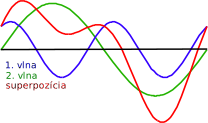
\includegraphics{obrazky/optika/interferencia_1}
 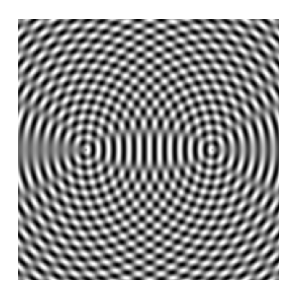
\includegraphics{obrazky/optika/interferencia_2}

 \caption{Interferencia 2 vĺn a) na priamke b) na ploche}
 \label{fig:interferencia}
 \end{figure}

Pre jednoduchosť budeme uvažovať interferenciu monochromatických vĺn.
Prax ukazuje, že zaujímavá vie byť aj všeobecná interferencia,
napríklad farebné sfarbenie povrchu bublín či olejových škvŕn, ale
táto téma je už nad rámec tejto publikácie.

Zoberme teda zdroj (skalárneho) vlnenia v 3-rozmernom priestore.
Ak je poloha zdroja $\vect{a}$, amplitúda $A$, počiatočná fáza $\phi$ a vlnová dĺžka
$\lambda$, tak v čase $t$ bude v mieste $\vect{r}$ výsledná amplitúda rovná

\begin{equation}
X(\vect{r},t)=A \sin(2 \pi \frac{|\vect{r}-\vect{a}| - t c}{\lambda}+\phi)
\end{equation}

Podľa princípu superpozície pre $N$ zdrojov $1,\dots,N$ platí
\begin{equation}
X(\vect{r},t)=\sum_{i=1}^{N} A_i \sin(2 \pi
\frac{|\vect{r}-\vect{a_i}| - t c}{\lambda}+\phi_i)
\end{equation}

Na tomto mieste si povieme niečo o objektoch zvaných komplexné
amplitúdy.

\definicia{Komplexná amplitúda}{
Nech má vlna amplitúdu $A$ a fázu $\phi$.
Pod pojmom komplexná amplitúda budeme rozumieť komplexné číslo
$\mathcal{A}=A e^{i \phi}$.
}


Lema: Reálna časť komplexnej amplitúdy je amplitúda vlny v danom bode.
Dôkaz: Komplexná amplitúda je vlastne obohatenie pôvodného vzorca o
imaginárnu časť.


Lema: Energia prislúchajúca vlne je $E \thickapprox A^2$.

Definicia: Nech $a$ je amplitúda vlny s periódou $p$. 
Potom priemerná energia $E_p \thickapprox \frac{1}{p} \int_0^p a(x)^2 dx$.

\begin{poznamka}
 Našim cieľom bude zhodnotiť energiu rýchlo kmitajúcej vlny.
 Čitateľ si tak môže všimnúť analógiu tohoto deja s elektrickou
 energiou. Keď máme jednosmerný obvod, energia ktorá sa spotrebúva
 napríklad na rezistore je časovo konštantná. Naproti tomu za
 prítomnosti striedavého napätia táto energia (za jednotku času) kolíše
 a v praxi nás zaujíma len jej stredná hodnota. To isté môžeme
 uvažovať aj u svetla, kedy nás nezaujíma energia (resp.
 pravdepodobnosť výskytu fotónov z kvantovej mechaniky) 
 na danom mieste v konkrétnom čase,
 ale jej stredná hodnota, lebo to je veličina ktorú vieme merať.
\end{poznamka}

Veta: Priemerná energia sínusovej vlny s komplexnou amplitúdou
$\mathcal{A}$ $E_p \thickapprox |\mathcal{A}|^2$.
Dôkaz:
$E_p \thickapprox \frac{c}{\lambda} \int_0^{\lambda/c}
(A \sin(2 \pi \frac{L - t c}{\lambda}+\phi))^2
= A^2 \frac{c}{\lambda} \frac{\lambda}{2 c} =
\frac{1}{2} A^2 = \frac{1}{2} \mathcal{A}^2$.

\todo{pokracovanie}

    \subsection{Spektrálna analýza}

Snáď najdôležitejšou aplikáciou fourierovej transformácie vo fyzike a
chémii je spektrálna interferometria. V tejto kapitole v skratke
rozvedieme najdôležitejšie pojmy a mechanizmy o tejto pre chemikov
životne dôležitej metóde skúmania látok.


Ako už názov naznačuje, spektrálna analýza má za úlohu analyzovať
látky. Deje sa tak prostredníctvom infračervených vĺn. Čitateľ by sa
mohol opýtať, prečo sa používajú tieto vlny a jeho zvedavosti bude za
chvíľu zadosťučinené.

\subsubsection{Chemické väzby}

Základom každej chemickej zlúčeniny sú atómy, medzi ktorými vznikajú
väzby. Väzba je akási neviditeľná pružina, ktorá vzniká ako dôsledok
pôsobenia elektromagenetickej a slabej jadrovej sily. Existuje istá
vzialenosť molekúl, keď sú tieto sily v rovnováhe a celková energia
väzby je minimálna. Vychýlením atómu zo svojej polohy prevládne jedna
z týchto dvoch síl a atóm má snahu dostať sa do svojej pôvodnej
polohy. Samozrejme, atómy za predpokladu bežnej teploty nestoja na
mieste ale kmitajú okolo rovnovážnej polohy a väzby ich držia pokope.

To čo je ale pri spektrálnej analýze dôležité je, že rôzne väzby sa
správajú rôzne. Kratšie väzby kmitajú rýchlejšie, väzba od ťažkých
atómov kmitá pomalšie, a takisto vlastnosti väzby závisia aj od
elektrických vlastností atómov. Preto sa každá väzba dá identifikovať
podľa svojej frekvencie kmitania. Prehľad niektorých vybraných typov
väzieb a k nim prislúchajúcich frekvencií sa dá nájsť v tabuľke 
\ref{tab:vazby} (čiastočne prevzaná z \cite{wiki:spectro}).
Po nahliadnutí do tabuľky by nám už malo byť jasné, odkiaľ dostala
spektrometria prívlastok infračervená - infračervené (tepelné) lúče
majú vlnovú dĺžku medzi 750nm a 1mm.

\begin{table}[htb]
    \centering
    \begin{tabular}{| l | r | r |}
        \hline
        väzba & špecifický typ väzby & vlnová dĺžka $\cm^{-1}$ \\ \hline
        C-O & alkoholy & 1040-1060, 1100 \\ \hline
        C-H & C=CH & 3020 \\ \hline
        C-H & metyl & 1260 \\ \hline
        C=O & aldehyd & 1725 \\ \hline
        C-C & aromatické C=C & 1450, 1500, 1580, 1600 \\ \hline
        O-H & alkoholy & 3200-3400 \\ \hline
        N-H & amíny & 3400-3500, 1560-1640 \\ \hline
    \end{tabular}
    \caption{Ukážka absorbčných frekvencií väzieb}\label{tab:vazby}
\end{table}

Otázkou teda ostáva, ako odhaliť frekvenciu kmitania väzieb. Odpoveď
nám núka fyzika sama. Atómy sa bežne nachádzajú v základnom stave.
Avšak pôsobením žiarenia s frekvenciou rovnou frekvencii kmitania
väzby môžeme atóm rozkmitať ešte viac. Je to jav podobný rezonancii - 
vonkajším pôsobením vynútime kmity rezonátora - väzby.
Takto rozkmitaný atóm sa môže dostať do excitovaného stavu. Pri tomto
prechode medzi stavmi atóm pohltí energiu. Zo zákona zachovania
energie musí tým pádom dopadajúce žiarenie stratiť nejakú časť
energie. No a táto strata energie (na príslušnej frekvencii) je
základom pre spektrometriu.


\begin{poznamka}
    Viac o chemických väzbách sa dá nájsť v \cite{wiki:bonds} a
    \cite{Chem}. Taktiež na stránke \cite{webspectra} sa dá nájsť
    interaktívny program na porovnávanie spektier.
\end{poznamka}

\subsubsection{Konštrukcia spektrometra}

Spektrometer môžeme rozdeliť na niekoľko základných častí.
\begin{itemize}
    \item zdroj IR žiarenia 
    \item Michaelsonov interferometer - zložený z takzvaného
    ``beamsplittera'' čo je polopriepustné zrkadlo, jedného fixného
    a jedného pohyblivého zrkadla
    \item kryštál
    \item detektor
\end{itemize}
Zjednodušenú schému spektrometra možno vidieť na obrázku
\ref{fig:ftir_schema}

\begin{figure}[htp]
    \centering
    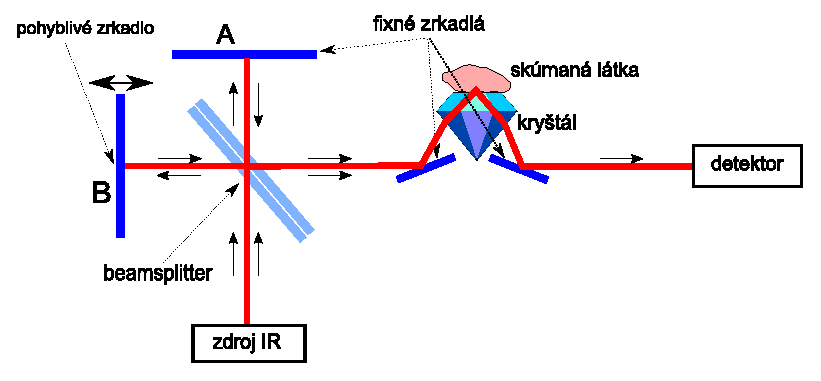
\includegraphics{obrazky/fyzika/ftir/ftir_schema}
    \caption{Základná konštrukcia spektrometra}\label{fig:ftir_schema}
\end{figure}

Infračervený lúč začne svoju púť v zdroji žiarenia. Obvylke je to 
cievka, ktorá je napájaná jednosmerným napätím a zohrieva sa.
Potom, ako lúč opustí zdroj, narazí na beamsplitter. Beamsplitter
je IR priehľadný materiál, napríklad bromid draselný (KBr). 
Beamsplitter pôsobí
na lúč ako polopriehľadné zrkadlo. Približne jednu polovicu žiarenia
prepustí smerom na zrkadlo A, druhú polovicu smerom na zrkadlo B.
Žiarenia odrazené od zrkadla A sa opäť dostáva do beamsplittera,
časť pokračuje smerom ku kryštálu a časť sa vracia do zdroja.
Žiarenie odrazené od zrkadla B sa taktiež dostáva do beamsplittera a
opäť jedna časť sa vráti do zdroja a druhá časť pokračuje v smere na
kryštál. Nás bude odteraz zaujímať iba žiarenie smerujúce do kryštálu.
Toto žiarenie je zložením dvoch lúčov z toho istého zdroja, avšak
(vďaka tomu, že zrkadlo B je pohyblivé) tieto lúče majú istý
dráhový rozdiel. Lúče preto spolu interferujú a môžeme
uvažovať, ze ďalej pokračuje len jeden výsledný lúč.
Tento je pomocou zrkadiel nasmerovaný do kryštálu. Kryštál má zaistiť,
aby sa lúč dostal do povrchovej vrstvy látky, od nej sa odrazil a
pokračoval ďalej k detektoru. V detektore sa zachytený signál
premení na elektrické napätie.


\subsubsection{Výpočet absorpcie}

\begin{definicia}[Transmitancia]
    $T=I/I_0$ je podiel prepusteného žiarenia látkou k dopadajúcemu
    žiareniu
\end{definicia}

\begin{definicia}[Absorbcia]
    Absorbciou budeme označovať logaritmickú škálu transmitancie,
    $A=-\log_{10}T$
\end{definicia}

Základom pre chemickú analýzu je graf $A(f)$ absorbcie materiálu v
závislosti od frekvencie. 

Celkovo môžeme teda písať, že $A(f) = -\log_{10} \frac{I(f)}{I_0(f)}$.
Problém ale ostáva v určovaní $I(f), I_0(f)$. Detektor totiž nevie rozlíšiť
žiarenia jednotlivých frekvencií ale mieša ich všetky dokopy.

\begin{poznamka}
    Existujú aj detektory, ktoré vedia rozlišovať intenzitu podľa
    frekvencie. Poväčšinou ale fungujú tak, že na vstupe detektora sa
    žiarenie nasmeruje do hranola, ktorý podobne ako v prípade svetla
    žiarenie rozloží na jednotlivé monochromatické časti a následne
    sa môže merať intenzita iba konkrétnej frekvencie. Základy možno
    nájsť na \cite{wiki:spectrometer} a komu by nestačilo, tak viac o tejto
    spektrometrii sa dá dočítať v \todo{}. 
\end{poznamka}



Výsledok ktorý odčítame z detektora je jediná hodnota 
$I=\int_0^\infty I(f) df$
\footnote{Presnejšie povedané výsledkom nie je intenzita ale energia.
Tieto 2 veličny sú ale priamo úmerné a tak je jednoduché určiť
"intenzitu"}.

Aby sme mohli z $I$ určiť $I(f)$, musíme použiť nasledujúci trik.

Nech $I(x)$ je hodnota nameraná detektorom, ak je zrkadlo B vo
vzdialenosti $x$ od beamsplittera. Pre našu pohodlnosť si ešte zavedieme,
že $x$ sa meria smerom zľava doprava. Ďalej nech $y$ je vzdialenosť zrkadla
A od beamsplittera a nech $I_z(f)$ je intenzita žiarenia o frekvencii
$f$ zdroja. Predpokladajme, že beamsplitter rozdelí žiarenia na 2 lúče
a po ďalšom prechode cez beamsplitter dostaneme lúče 
približne rovnakej intenzite. Môžeme písať
\begin{align}
    I_{z_1}(f,t) = a_1(f) \cos (2 \pi f (t+2x) + \phi) \\
    I_{z_2}(f,t) = a_2(f) \cos (2 \pi f (t+2y) + \phi) \\
\end{align}
kde $\phi$ je fáza vstupujúceho žiarenia do beamsplittera a $t$ je
vzdialenosť od beamsplittera v ktorej meriame požadovanú intenzitu a
$a_1,a_2$ sú konštanty kombinujúce pôvodnú intenzitu zdroja a
priepustnosť beamsplittera pre oba lúče.
Podľa lemy \ref{lema:lk_harmonickych_funkcii} môžeme tvrdiť, že
interferenctiou vznikne
\begin{equation}
    I_{z}(f,t,x) = a(f) \cos (2 \pi f (t+2x) + \psi)
\end{equation}
Potom detektor vo vzdialenosti $t$ zachytí intenzitu

\begin{align}
    I(x,t)=\int_0^\infty I_z(f,t,x) T(f) \dd f \\
    I(x,t)=\int_0^\infty T(f) a(f) \cos(2 \pi f (t + 2x) + \psi) \dd f
\end{align}
Posledná rovnica dáva ale nádej na zvrat v situácii. Pre fixné
$t$\footnote{A detektor je fo fixnej vzdialenosti} 
je to totiž Fourierova transformácia obohatená o posunutie a iné
nepríjemnosti. Faktom ale ostáva, že nie je veľký problém pár
substitúciami a rozšírením integrácie pomocou symetrie na celé $\R$
dostať štandardnú fourierovu transformáciu funkcie $I(f) = T(f) a(f)$.
Potom ale vieme spraviť spätnú transformáciu a z hodnôt $I(x)$
vypočítať $I(f)$.
\begin{poznamka}
    Jeden by mohol namietať, že nemôžeme zmerať
    $I(x)$ na celej množine $R$. Za rozumných predpokladov, akými sú
    žiarenie detektora len v istom frekvenčnom pásme,
    vieme obmedziť hranice integrácie na konečné hodnoty.
\end{poznamka}

Základom spektrálnej analýzy je teda nameranie $I(x)$ na istom
intervale a následné vypočítanie inverznej transformácie. Veľká výhoda
tejto metódy spočíva vo fakte, že jediná pohyblivá súčiastka je jedno
zrkadlo beamsplittera a teda realizácia je konštrukčne nenáročná.
Detektor navyše vieme jednoducho nakalibrovať meraním prázdnej vzorky.

    \subsection{Kvantová mechanika}
\subsubsection{Heisenbergova nerovnosť}

Táto nerovnosť hovorí, že pre ľubovoľný signál je nemožné aby bol
naraz spektrálne a časovo ohraničený.
Aby sme zaviedli presnejšie kvantitatívne vyjadrenie, zavedieme si pojem
disperzie funkcie okolo bodu.

%%% {{{ definicia disperzie
\def\disperzia#1{\mathcal{D}_{#1}}
\begin{definicia}
    Dispezriou funkcie $f \in \LLinf, f \not = 0$ okolo bodu $a$ nazveme
    \begin{equation}
        \disperzia{a} f = \frac{\int (x-a)^2 |f(x)|^2 \dd x}
                               {\int |f(x)|^2 \dd x}
    \end{equation}
\end{definicia}
\begin{poznamka}
    Pozornejší čitatelia si mohli všimnúť, že takto definovaná
    disperzia je prirodzeným rozšírením definície disperzie funckie
    $|f(x)|^2$ v štatistike
\end{poznamka}

Interpretácia disperzie je akási miera neschopnosti funkcie byť
koncentrovanou okolo istého bodu. Pokiaľ $f$ dosahuje význačné hodnoty
len v tesnom okolí $a$, tak $\disperzia{a}f$ je malá. Naopak, ak
$f$ má význačnú časť ďaleko od $a$, disperzia bude veľká.
%%% }}}

%%% {{{ Heisenbergova nerovnost
\begin{lema}
    \begin{equation}
        \disperzia{a}f > 0
    \end{equation}
    \label{lema:nenulova_disperzia}
\end{lema}
\begin{dokaz}
    Vieme, že $f\not=0$ a preto $0 \not=\int |f(x)|^2 \dd x <\infty$.
    Nerovnosť je teda ekvivalentná s
    \begin{equation}
        \int (x-a)^2 |f(x)|^2 \dd x > 0
    \end{equation}
    Predpokladajme naopak, že ľavá strana je rovná nule (je zjavné, že
    nemôže byť záporná). Potom
    \begin{equation}
    \begin{split}
     0 = & \int (x-a)^2 |f(x)|^2 \dd x \\
         =& \int x^2 |f(x+a)|^2 \dd x \\
         =& \int (x |f(x+a)|)^2 \dd x
    \end{split}
    \end{equation}
    Dostali sme teda, že $x|f(x+a)|$ je rovná nule skoro všade.
    Tým pádom ale musí platiť aj $|f(x+a)|=0$ skoro všade, čo je 
    v spore s tým, že $f$ je nenulová funkcia.
\end{dokaz}

Nasledujúca veta tvrdí, že $f$ a $\dual{f}$ nemôžu byť obe
koncentrované okolo bodov.

\begin{veta}
    Heisenbergova nerovnosť:
    Pre $\forall f\in \LLinf \land f\in \PSinf$ platí
    \begin{equation}
        (\disperzia{a}f)(\disperzia{\alpha}\dual{f}) \ge \frac{1}{4}
        \quad \text{pre všetky } a,\alpha \in \R
        \label{eq:hei_ineq}
    \end{equation}
\end{veta}
\begin{dokaz}
    Začnime prípadom $a=\alpha=0$.
    Predpokladajme $x f(x) \in \LLinf$ a $f'(x)\in \LLinf$.
    V prípade že $x f(x) \not\in\LLinf$, máme
    $\int x^2 |f(x)|^2 \dd x = \infty$ a teda $\disperzia{0}f=\infty$.
    Podobne, podľa \todo{} vieme (s predpokladmi $f \in \LLinf \land
    f' \in \PCinf$) že platí ekvivalencia $f'(x)\in\LLinf \equiv
    y\dual{f}(y)\in\LLinf$ ak $f'(x)\not\in\LLinf$. Potom ale 
    $y\dual{f}(y) \not\in\LLinf$ a teda $\disperzia{0}f'=\infty$.
    V oboch spomínaných prípadoch nerovnosť triviálne platí nakoľko
    podľa lemy \ref{lema:nenulova_disperzia} disperzia je nenulová.

    Pokračujme v práci - majme funkciu $x\conjug{f(x)}f'(x)$, ktorá patrí $\PCinf$. 
    Integráciou per-partes na intervale $(a,b)$ dostaneme
    \begin{equation}
        \int_a^b x\conjug{f(x)}f'(x) \dd x =
          \left[ x|f(x)|^2\right]_a^b -
          \int_a^b \left(|f(x)|^2 + x f(x) \conjug{f(x)} \right)
            \dd x
    \end{equation}
    resp.
    \begin{equation}
    \begin{split}
        \int_a^b |f(x)|^2 \dd x &=
          \left[ x|f(x)|^2\right]_a^b 
        - \int_a^b x\conjug{f(x)}f'(x) \dd x -
          \int_a^b x f(x) \conjug{f'(x)} \dd x \\
        &= \left[ x|f(x)|^2\right]_a^b 
        - \int_a^b x\conjug{f(x)}f'(x) + x f(x) \conjug{f'(x)} \dd x
          \\
        &= \left[ x|f(x)|^2\right]_a^b 
        - \int_a^b \conjug{x} \conjug{f(x)}f'(x) + x f(x)
          \conjug{f'(x)} \dd x\\
        &= \left[ x|f(x)|^2\right]_a^b 
        - 2 \Re \int_a^b \conjug{xf(x)}f'(x) \dd x
    \end{split}
    \end{equation}
    Pretože $f(x),x f(x), f'(x)$ sú v $\LLinf$, limity integrálov
    v rovnici ak $a\imply-\infty$ a $b\imply\infty$ existujú.
    Preto musia existovať aj limity $a |f(a)|^2, b |f(b)|^2$ a musia
    byť nulové. Inak by muselo platiť
    $f(x)\sim\frac{c}{\sqrt{|x|}}$ a $f$ by nemohla byť v $\LLinf$.
    Limitovaním do nekonečna potom dostaneme
    \begin{equation}
        \int |f(x)|^2 \dd x= - 2 \Re \int \conjug{x f(x)}f'(x) \dd x
        \label{eq:hei_before_cauchy}
    \end{equation}
    Podľa \todo{ref; cauchy} Cauchy-Schwarzovej nerovnosti
    \begin{equation}
        |\int \conjug{x f(x)}f'(x) \dd x| \le
            \left( \int x^2 |f(x)|^2 \dd x \right)^2
            \left( \int |f'(x)|^2 \dd x \right)^2
        \label{eq:hei_cauchy}
    \end{equation}
    A skombinovaním \ref{eq:hei_before_cauchy} s \ref{eq:hei_cauchy}
    dostaneme
    \begin{equation}
        \left( \int |f(x)|^2 \dd x)\right)^2 \le 4
            \left( \int x^2 |f(x)|^2 \dd x \right)
            \left( \int |f'(x)|^2 \dd x \right)            
        \label{eq:hei_after_cauchy}
    \end{equation}
    Podľa \todo{perseval's theorem} platí
    $\int |f(a)|^2 \dd a = \frac{1}{2\pi} \int |\dual{f}(\alpha)|^2 \dd
    \alpha$ a tiež \todo{derivative theorem}
    \begin{equation}
        \int |f'(x)|^2 \dd x = \frac{1}{2 \pi}
            \int |\fourier[f'](\chi)|^2 \dd \chi = 
            \frac{1}{2 \pi} \int \chi^2 |\dual{f}(\chi)|^2 \dd \chi
    \end{equation}
    Rovnicu \ref{eq:hei_after_cauchy} tak možno prepísať na
    \begin{equation}
        \left( \int |f(x)|^2 \dd x \right)
        \left( \int |\dual{f}(\chi)|^2 \dd \chi \right)
        \le 4
        \left(\int x^2 |f(x)|^2 \dd x \right)
        \left(\int \chi^2 |\dual{f}(\chi)|^2 \dd \chi\right)
    \end{equation}
    Čo je presne rovnica \ref{eq:hei_ineq} pre $a=\alpha=0$ ak uvážime že
    $f\not=0$ a tiež $\dual{f}\not=0$ \footnote{Samozrejme v $\LLinf$}.
    Všeobecný prípad ľahko prevedieme na záver pre nulové $a,\alpha$
    nasledujúcim spôsobom.
    Položme
    \begin{equation}
        g(x) = e^{-\imag \alpha x} f(x + a)
    \end{equation}
    \todo{this} Ľahko nahliadneme, že $\disperzia{a} f = \disperzia{0}g$ a 
    $\disperzia{\alpha}\dual{f} = \disperzia{0}\dual{g}$.
\end{dokaz}
%%% }}}


    \subsection{Analýza RLC obvodov}

RLC analýza je analýza obvodov zložených z odporov, kondenzátorov a
cievok. Tieto rezonančné obvody hrajú dôležitú úlohu vo fyzike.
Základným krokom, ktorý nám umožní ich analýzu pomocou Fourierovej
transformácie je princíp superpozície
\begin{veta}[Princíp superpozície]
 Nech $U_1(t), I_1(t)$ a $U_2(t), I_2(t)$ sú dve riešenia RLC obvodu
 \footnote{Pod pojmom riešenie myslíme "riešenie sústavy
 diferenciálnych rovníc popísaných daným obvodom"}.
 Potom $U(t)=a_1 U_1(t) + a_2 U_2(t), I(t)=a_1 I_1(t) + a_2 I_2(t)$ je
 tiež riešením daného obvodu
\end{veta}
\begin{dokaz}
    Načrtneme si základné črty dôkazu, nepôjdeme však do podrobností.
    Každý RLC obvod vieme popísať ako sústavu diferenciálnych rovníc - 
    jedna rovnica pre vzťah napätia a prúdu na každej súčiastke +
    rovnice pre všetky uzly, ktoré popisujú nemožnosť hromadenia sa
    náboja na jednom mieste.
    Rovnice pre jednotlivé súčiastky
    \begin{itemize}
        \item Rezistor: $U(t) = R I(t)$
        \item Kondenzátor: $I(t) = C \pd{U}{t}$
        \item Cievka: $U(t) = L \pd{I}{t}$
        \item Uzol: $\sum_{k} I_k(t) = 0$
    \end{itemize}
    Všetky tieto 4 typy diferenciálnych rovníc majú spoločnú vlastnosť
    - linearitu medzi napätím a prúdom. Nie je tažké overiť, že pre ne
      platí princíp superpozície. Potom ale platí princíp superpozície
      pre celú sústavu týchto rovníc a teda pre RLC obvod.
\end{dokaz}
\begin{poznamka}
    Čitateľ mohol nadubodnúť dojem, že superpozícia u obvodov je
    evidentná. Veľmi rýchlo ho ale vyvedieme z omylu. Už len taká
    jednoduchá súčiastka ako dióda je prudko nelineárna. Ideálna dióda
    prepúšťa prúd len jedným smerom. Aplikáciou princípu superpozície
    dvoch prúdov rovnakej veľkosti ale opačného smeru by sme ľakho
    mohli dospieť k záveru, že za nulového prúdu tečúceho obvodom
    tečie nenulový prúd diódou. Zjavný spor. Superpozícia preto nie je 
    \todo{allmighty} nástroj na riešenie všetkých elektrických obvodov
\end{poznamka}

Podobne ako v prípade optiky, zavedieme si pojem komplexnej amplitúdy.

\todo{lit:}
%http://www.google.com/url?sa=U&start=5&q=http://www.eas.asu.edu/~holbert/eee202/EEE202_Lect12_DiffEqSolutionTransientCircuits.ppt&ei=XhjPSbXxC8HF_Qbnj_3yCQ&sig2=6yYiVDxQt1Nq3jTpLBUm5Q&usg=AFQjCNGVag3OJgkQIbwCUy_fRgBD02Y_Zw

    
\section{Informatika}
    \subsection{Signal processing}

Či chcete alebo nechcete, signal processing je veľmi dôležitou
súčasťou každodenného života. Okolo nás sa každú sekundu prenesú veľké
množstvá údajov rôzneho typu. A práve tu hrá životne dôležitú hereckú
rolu konverzia analógového a digitálneho signálu. Vysielanie
televízie, rádia, alebo rozprávanie sa modemov, to všetko sú analógové
signály, ktoré treba nejakým spôsobom preniesť do digitálneho sveta. V
rannej dobe boli technológie čisto analógové, ale v dnešnej dobe sa
stretávame s náročným digitálnym spracovaním. Či ide o záznam zvuku
mikrofónom alebo meranie napätia voltmetrom, všade sa vynára tá istá
otázka.

\subsubsection{Je možné digitalizovať analógový signál?}
Odpoveď je nie. Nie bez ďalších predpokladov. Signál môže byť
ľubovoľný a nech by sme akokoľvek rýchlo zaznamenávali, stále nemusíme
zaznamenávať dostatočne rýchlo. Taktiež nemôžeme zaznamenávať s
nekonečnou presnosťou. Toto sú limitujúce faktory, ktoré prekážajú
záznamu signálu. Zaoberajme sa preto otázkou, či za nejakých
zjednodušených predpokladov je možné rekonštruovať signál iba z
čiastočných údajov. Možno je to prekvapujúce, ale dá sa to. Základ
tejto teórie vypracovali páni Nyquist a Shannon. Sformulujme a dokážme
si preto jednu základnú vetu zo signal processingu.

\begin{veta}
    (Nyquist-Shannon sampling theorem) Nech $f(x)$ je ľubovoľná
    funkcia z $\LLinf$. Ak $\exists B$ také že $f$ je bandlimited
    frekvenciou $B$, tak postačujúcou podmienkou
\end{veta}

    % vim:spell spelllang=sk
\subsection{Signal processing - digitálne filtre}
%% {{{
Digitálne filtre sú dôležitou súčasťou spracovania digitálneho
signálu. Podobne ako analógové filtre, ich úlohou je zo vstupného
signálu vybrať pre nás podstatnú časť, prípadne ju zosilniť alebo inak
modifikovať signál. V tomto dokumente si spomenieme niekoľko 
najzákladnejších filtrov používaných v praxi a súvisiacich s Fourierovou
transformáciou. Budeme ich demonštrovať na spracovaní obrazu, hoci
mnohé z nich sú viac dôležité v spracovaní zvuku/signálu 
\footnote{V elektronickej prílohe je možné nájsť aj demonštráciu 
týchto filtrov pre zvuk, v publikovanej podobe z pochopiteľných
dôvodov nie je
}.
Najskôr si popíšeme filtre pracujúce vo frekvenčnom rozsahu, potom
spomenieme filtre pracujúce na \todo{spatial} dátach a kapitolu
zavŕšime ukázaním súvisu medzi týmito dvoma prístupmi a
dekonvolúciou, ktorá sa snaží invertovať následky nežiadúcich filtrov.
%% }}}

\subsubsection{Ideálny lowpass a highpass filter}
Ideálny lowpass a highpass filter o limitujúcej frekvencii $f$ môžeme
popísať obrázkom \ref{fig:ideal_lowpass}, kde na $x$-ovej osi je frekvencia
vstupného signálu a na $y$-ovej osi je hodnota výstupného signálu.
\begin{poznamka}
    Väčšina filtrov vo frekvenčnej oblasti sa dá popísať podobným grafom.
    Čitaťeľ ale musí brať ohľad na istú nepresnosť - daný graf
    nešpecifikuje presne filter. Špecifikuje len zmenu amplitúdy.
    Bežné filtre fázu nemenia a preto sa ticho predpokladá $\phi(f)=0$.
\end{poznamka}

\begin{figure}[htp]
    \centering
    \includegraphics{obrazky/informatika/signal_processing/ideal_lowpass}
    \includegraphics{obrazky/informatika/signal_processing/ideal_highpass}
    \includegraphics{obrazky/informatika/signal_processing/ideal_lowpass_3d}
    \includegraphics{obrazky/informatika/signal_processing/ideal_highpass_3d}
    \caption{Frekvenčná priepustnosť ideálneho lowpass a highpass filtru}
    \label{fig:ideal_lowpass}
\end{figure}

Dané filtre prepúšťajú všetky frekvencie na jednu stranu od hraničnej
a na druhú stranu neprepustia nič. Ako si ukážeme vizuálne, tieto
filtre majú spoločný problém - "znovenie". Najvýraznejšie sa prejavuje
práve pri highpass filtri. Preto sú v praxi nepoužiteľné. Zvonenie
pochádza práve z ich ideality - obrazom jedného obrazového bodu, resp.
kruhu je sada sústredných kružníc a keď vymažeme všetky kružnice od
nejakej frekvencie, pri spätnej transformácii budú chýbať. Toto
zvonenie úzko súvisí s Gibbsovým fenoménom, ktorý sme už skúmali v
\todo{}. V praxi sa preto viacej používajú hladké filtre.

\begin{figure}[htp]
    \centering
%    \includegraphics{obrazky/informatika/signal_processing/ideal_lowpass}
    \caption{Ideálny lowpass filter}
    \label{fig:ideal_lowpass_image}
\end{figure}


\begin{figure}[htp]
    \centering
%    \includegraphics{obrazky/informatika/signal_processing/ideal_lowpass}
    \caption{Ideálny highpass filter}
    \label{fig:ideal_highpass_image}
\end{figure}


\subsubsection{Hladké filtre}
Ako sme v predchádzajúcej sekcii ukázali, ideálne filtre majú zvoniaci
efekt. Preto sa v praxi používajú filtre, ktoré majú spojitý a hladký
prechod medzi frekvenciami, ktoré filtrujú a frekvenciami, ktoré
nefiltrujú. Ukážeme si 2 rôzne filtre - Butterworth a Gaussov.



\subsubsection{Súvis medzi frekvenčnými a \todo{spatial} filtrami}
Klasické \todo{spatial}

\subsubsection{Gaussian ako iterovany median}

    \subsection{Image processing}

Táto kapitola bude venovaná spracovaniu obrazovej informácie a ako sa
pri tom dá využiť Fourierova transformácia. Ukážeme si dôležitosť
magnitúdy a fázy, rýchle hľadanie patternu rovnakej
veľkosti a orientácie a watermarking. O digitálnych filtroch pre
obrazovú informáciu sme už písali v predchádzajúcej kapitole a tak ich
láskavo preskočíme.

\subsubsection{Fourierova transformácia - fáza a magnitúda}


\subsubsection{Hľadanie patternov}
Jednou z nečakaných aplikácii konvolúcie je aj takzvaný korelačný
filter. Korelácia sa používa na identifikáciu

\subsubsection{Watermarking}

    % vim:spell spelllang=sk
%\subsection{Image compression}
\section{Image compression}

%% {{{ zakladny nacrt kompresie
%\subsubsection{Základný náčrt kompresie údajov}
\subsection{Základný náčrt kompresie údajov}
Stratová (ale aj bezstratová) kompresia údajov je založená na
jednoduchých princípoch. Jej hlavné črty si môžeme popísať v troch
krokoch
\begin{itemize}
\item Transformácia
\item Kvantizácia
\item Kompresia
\end{itemize}
Poďme sa bližšie zaoberať jednotlivými časťami.
Transformácia je bezstratová manipulácia s údajmi. Transformáciou môže
byť identita, rozdelenie obrazu na farebné zložky, zmena RGB na CMYK a
pod. Hlavnou úlohou transformácie je akosi predpripraviť dáta na
ďalšie spracovanie, dostať ich do vhodnej podoby pre ďalšie kroky, ale
pritom vedieť stále vypočítať reverznú transformáciu. Krok
transformácie je zároveň krokom, kedy sa nestrácia žiadna informácia.

Nasleduje, druhý krok, samotný krok zodpovedný za stratu informácie
pri stratovej kompresii. Pri bezstratovej kompresii je samozrejme
vynechaný. Výstupom z transformácie sú dáta. Tieto dáta môžeme
považovať za reálne resp. celé čísla. Ich problémom je veľká pamäť
potrebná na udržiavanie týchto informácii. Kvantizácia rieši tento
problém jednoducho inžiniersky - nejaké informácie vynecháme.
Spravidla sa to robí tak, že čísla sa vydelia kvantizačným faktorom a
zaokrúhlia nadol. Opačný proces ku kvantizácii môže len hádať pôvodné
čísla, preto je kvantizácia stratová. Je však na umení príslušného
spôsobu kvantizácie, aké to bude mať vizuálne následky. Ako vieme,
väčšina informácie skrytá v digitálnych obrázkoch či zvukoch je
takpovediac nepotrebná. Človek nemá natoľko vyvinuté zmysly aby ju
všetku videl/počul. Preto záleží len na šikovnosti, ktoré informácie
budú kvantizované viac a ktoré menej. Samozrejme, snahou je najviac
kvantizovať informácie pre človeka skryté a naopak, dôležité údaje
nekvantizovať vôbec. Tu si kvantizácia podáva ruku s predchádzajúcou
transformáciou - čím lepšie transformácia oddelí dôležité od
nedôležitého, tým lepšie vieme kvantizovať.

Poslednou časťou je kompresia. Toto je čiste bezstratová kompresia,
ktorá sa snaží ešte z kvantizovaných údajov vyžmýkať posledné voľné
bity a tak zavŕšiť finálnu podobu.

Príkladom formátu, ktorý nemá transformáciu, nemá kompresiu ale má
kvantizáciu je napríklad BMP - kvantizuje každú farebnú zložku do 8
bitov. Formátom bez transformácie s kvantizáciou a kompresiou môže byť
napríklad tga - prebieha v ňom Run-length kompresia, ktorá vie dobre
komprimovať dlhé úseky rovnakej farby.
V skutočnosti, najviac účinné formáty sú tie, ktoré používajú
sofistikovanú transformáciu. Príkladom je jpeg2000 využívajúci
waveletovú transformáciu či klasický formát jpeg. Práve pri ňom sa
teraz zastavíme a bližšie si popíšeme jeho kroky.
%% }}}

%% {{{ farebna predpriprava
%\subsubsection{Jpeg - farebná predpríprava}
\subsection{Jpeg - farebná predpríprava}
Dátový formát jpeg je sofistikovaný formát využívajúci viaceré
poznatky z vizuálneho vnímania obrazu.

V počítači je bežná reprezentácia farieb v takzvanom RGB móde, kde
farba pozostáva z koordinátov v 3D priestore (Červená, Zelená, Modrá).
Hoci je tento spôsob veľmi intuitívny pre CRT monitory, nie je
perfektný pre kompresiu. Trojica farieb červená, zelená a modrá totiž
nepopisuje spôsob vnímania ľudskou bytosťou rovnomerne. Formát jpeg
rieši tento problém zavedením nového farebného priestoru $(Y,Cb,Cr)$,
ktorý sa dá vypočítať nasledovne \footnote{Prevzaté z \cite{jfif}} 
(predpokladáme 8-bitové RGB hodnoty)
\begin{align*}
    Y &= 0.299 R + 0.587 G + 0.114 B \\
    Cb &= -0.1687R - 0.3313G + 0.5B + 128 \\
    Cr &= 0.5R - 0.4187 G - 0.0813B + 128
\end{align*}
Pričom spätná transformácia je
\begin{align*}
    R &= Y + 1.402 (Cr - 128) \\
    G &= Y - 0.34414 (Cb-128) - 0.71414 (Cr-128) \\
    B &= Y + 1.772 (Cb - 128)
\end{align*}
Nasleduje prvá kvantizácia nazývaná Chroma subbampling, 
kde sa zložky  $Cr, Cb$ redukujú na nižšie
rozlíženie. Ľudské oko je totiž omnoho menej citlivé na zmenu farby
ako na zmenu jasu. Pri kompresii si preto môžeme dovoliť zmenšiť
rozlíšenie s akým je uchovaná farba.
Nepríjemným vedľajším dôsledkom môže byť "pretekanie" farebného
odtieňa na silno kontrastných hranách.
\begin{poznamka}
Viac o subsamplingu sa čitateľ môže dozvedieť v 
\todo{wiki}%http://en.wikipedia.org/wiki/Chroma_subsampling}
\cite{subsampling}
\end{poznamka}
%% }}}


%% {{{ DCT
%\subsection{Jpeg - kosínová transformácia}
\subsection{Jpeg - kosínová transformácia}

Po tejto úprave sa všetky tri vrstvy spracúvajú samostatne a tým
istým spôsobom. Snahou je zredukovať ďalšiu nepotrebnú informáciu.
Práve tu sa ujíma vedenia Fourierova transformácie, presnejšie
povedané jej kamarátka diskrétna kosínová transformácia. Jej špeciálna
verzia pre JPEG sa od vzorca \ref{eq:dct_transform} 
líši normalizáciou a špecializáciou na vstup veľkosti 8x8.
\begin{equation}
   F(u,v) = \frac{1}{4} C(u) C(v) 
    \sum_{x=0}^7 \sum_{y=0}^7 f(x,y)
        \cos\frac{(x+1/2) u \pi}{8}
        \cos\frac{(y+1/2) v \pi}{8}
    \label{eq:dct_jpeg}
\end{equation}
Kde $C$ je definované ako
\begin{equation*}
    C(u) = \left\{
        \begin{array}{l l}
            \frac{1}{\sqrt{2}} & u=0 \\
            1 & u\not=0
        \end{array}
        \right.
\end{equation*}
Inverzná transformácia je definovaná ako
\begin{equation}
    f(x,y) = \frac{1}{4} 
        \sum_{u=0}^7 \sum_{v=0}^7 C(u) C(v) F(u,v)
        \cos\frac{(x+1/2) u \pi}{8}
        \cos\frac{(y+1/2) v \pi}{8}
    \label{eq:idct_jpeg}
\end{equation}
\begin{poznamka}
    Bolo by dobré upozorniť čitateľa na 2 zásadné rozdiely medzi
    kosínovou transformáciou a~jej inverznou transformáciou. Prvým je
    vyňatie $C(u) C(v)$ pred sumu v~rovnici \eqref{eq:dct_jpeg}
    narozdiel od rovnice \eqref{eq:idct_jpeg}, kde to nemôžeme spraviť.
    Druhým rozdielom je zhoda parametrov
    oboch kosínusov, navzdory intuícii, že inverzná transformácia by
    mala mať vymenené indexy $u,v$ s $x,y$
\end{poznamka}
Dôvod prečo je
diskrétna kosínová transformácia výhodnejšia si spomenieme neskôr,
nateraz si vysvetlíme princíp na ktorom si obe zakladajú. Ukazuje sa, že
ľudské oko je vnímavejšie v~oblasti nižších frekvencií. Presnejšie
povedané, omnoho viac vnímame svetlosť a~odtiene povedzme na veľkej
modrej ploche ako je obloha v~porovnaní s~rýchlo sa meniacimi farbami
morskej hladiny s~vlnami, kde sa prípadné zmeny spôsobené kompresiou
stratia. Diskrétna kosínová transformácia oddelí
jednotlivé frekvencie od seba, a~tak môžeme aplikovať rôznu
kvantizáciu pre rôzne frekvencie. Druhou výhodu tejto transformácie je
jej schopnosť sústreďovať väčšinu energie v~nízkofrekvenčnej oblasti.
Už bez samotnej kvantizácie vieme potom ušetriť na finálnej kompresii,
ktorá bude omnoho lepšie pracovať na údajoch, ktorých veľká časť má
nízku entropiu oproti vysokej entropii celého pôvodného signálu.
Obraz sa preto rozdelí na bloky veľkosti 8x8 pixelov, každý blok sa
spracúva samostatne.

Na daný blok sa najskôr aplikuje DCT podľa vzorca \ref{eq:dct_jpeg}.
Výsledok je opäť blok 8x8,
tentoraz vo frekvenčnom spektre. Môžeme si všimnúť, že maximálna
hodnota v~danom bloku môže byť väčšia ako je rozsah vstupných údajov,
transformáciu preto treba robiť s~väčším dátovým typom.
Dáta kvantizujeme a dekvantizujeme pomocou vopred určenej kvantizačnej matice $Q(u,v)$.
\begin{align*}
    F_Q(u,v) &= Round (F(u,v)/Q(u,v)) \\
    F'(u,v) &= F_Q(u,v) * Q(u,v)
\end{align*}

Ukážka prevodu pôvodného obrázku na kvantizované koeficienty 
a~spätná transformácia je v~tabuľke \ref{tab:jpeg_quantize}
%% }}}

%% {{{ tabulka kvantizacie
\begin{table}[htb]
    \centering
    \subtable[Pôvodné hodnoty]{
    \tiny
    \input tabulky/informatika/image_compression/original.tbl
    }

    \subtable[DCT]{
    \tiny
    \input tabulky/informatika/image_compression/after_dct.tbl
    }

    \subtable[Kvantizačné koeficienty]{
    \tiny
    \input tabulky/informatika/image_compression/quantization.tbl
    }
    \subtable[Po kvantizácii]{
    \tiny
    \input tabulky/informatika/image_compression/after_quantization.tbl
    }
    
    \subtable[Dekvantizácia]{
    \tiny
    \input tabulky/informatika/image_compression/after_dequantization.tbl
    }
    
    \subtable[Finálny výstup]{
    \tiny
    \input tabulky/informatika/image_compression/final.tbl
    }
    
    \caption{Postupná ukážka kvantizácie JPEG obrázku}
    \label{tab:jpeg_quantize}
\end{table}
%% }}}

%\subsubsection{Prečo DCT a nie DFT?}
\subsection{Prečo DCT a nie DFT?}
%% {{{ 
 V krátkosti si vysvetlíme základný rozdiel medzi Fourierovou a
 kosínovou transformáciou pri kompresii. Na prvý pohľad je totiž
 Fourierova transformácia výhodnejšia - ako sme už ukázali, výstup
 diskrétnej Fourierovej transformácie reálnych čísel je zbytočne
 veľký. V skutočnosti nám stačí si pamätať $\frac{1}{4}$ výstupu, pretože
 poznáme jeho symetriu v oboch rozmeroch. V spolupráci s predpokladom
 dvojnásobného počtu bitov na zapamätanie si komplexných čísel môžeme
 dôjsť k záveru, že výstup DFT je o polovicu menší ako výstup DCT.
 Tento záver je zjavne v niečom chybný, nakoľko by sme vedeli
 komprimovať ľubovoľné súbory na polovicu. Problém je v  presnosti -
 na výstup DFT potrebujeme väčšiu presnosť aby sme vedeli spraviť
 spätnú transformáciu. Toto ale nie je najhlavnejší dôvod prečo sa
 používa kosínová transformácia.

 Dôvod  prečo DCT a nie DFT si doslova ukážeme.
 Ide o schopnosť koncentrácie energie
 v menších frekvenciách. Z obrázka \ref{fig:dct_vs_dft}
 môžeme vidieť jemný rozdiel medzi týmito dvoma transformáciami
 Fourierova transformácia má najviac koeficientov s väčšou energiou
 ako diskrétna kosínová transformácia. Pri finálnej
 bezstratovej kompresii je to rozhodujúci fakt - kosínová
 transformácia má menej entropie a preto sa bude dať lepšie
 komprimovať.
%% }}}
%% {{{ fig:dct_vs_dft 
\begin{figure}[htp]
    \centering
    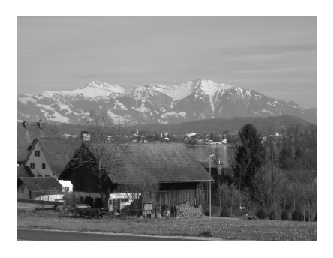
\includegraphics{obrazky/informatika/image_compression/image} \\
    
\includegraphics{obrazky/informatika/image_compression/dft}
    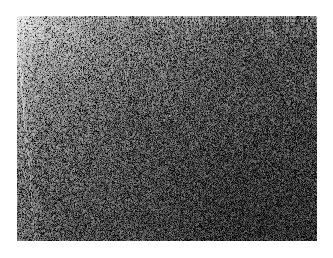
\includegraphics{obrazky/informatika/image_compression/dct} \\
    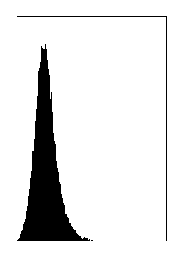
\includegraphics{obrazky/informatika/image_compression/dft_histogram}
    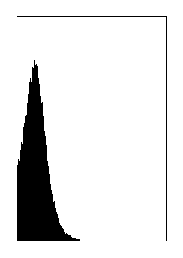
\includegraphics{obrazky/informatika/image_compression/dct_histogram}
    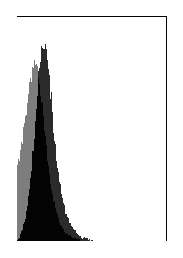
\includegraphics{obrazky/informatika/image_compression/combined_histogram}
    \caption{Porovnanie koncentrácie energie. Vľavo DFT, vpravo DCT,
    obrázok ukazuje normalizáciu koeficientov funkciou $\log 1+|x|$}
    \label{fig:dct_vs_dft}
\end{figure}
%% }}}


%\subsubsection{Jpeg kompresia }
\subsection{Jpeg kompresia }
\todo{entropy compression}
Nasleduje posledná fáza a~tou je kompresia. Kompresia bude fungovať
rôzne pre DC člen (0,0) a zvyšných 63 koeficientov. DC člen spravidla nesie v
sebe väčšinu energie a navyše je známe, že sa veľmi nemení medzi
susednými blokmi 8x8, preto sa počíta ako rozdiel od predchádzajúceho
DC člena. AC koeficienty sa najskôr zoradia do \todo{zig-zag}
postupnosti na obrázku \ref{fig:jpeg_zig_zag}. 

\begin{figure}[htp]
    \centering
    \includegraphics{obrazky/informatika/image_compression/zig_zag}
    \caption{JPEG formát - postupnosť v akej sú kódované AC koeficienty}
    \label{fig:jpeg_zig_zag}
\end{figure}

Zoradenie koeficientov
do tejto postupnosti je pomerne dôležité, pretože empiricky zoraďuje
najskôr najväčšie koeficienty a potom tie menšie až nulové.
Finálna kompresia je \todo{entropy coding}. Jpeg špecifikuje dva možné
pístupy - aritmetické kódovanie a Huffmanovo kódovanie. Aritmetické
kódovanie produkuje o 5-10\% lepšie výsledky, avšak je náročnejšie a
pre rýchle implementácie JPEGu sa používa spravidla Huffmanov kód.
Samotné Huffmanovo kódovanie nebudeme rozoberať v tejto publikácii,
po poznatkoch túžiaci čitateľ veľmi ľahko nájde literatúru na túto
tému.

%\subsubsection{Ďalšie aspekty JPEGu}
\subsection{Ďalšie aspekty JPEGu}

Existuje množstvo ďalších aspektov, ktoré sme v tomto krátkom úvode
nespomenuli, a stoja za zmienku. Existuje bezstratová verzia JPEGu,
ktorá funguje na úplne inom princípe. Navyše ukladanie dát je možné
rôznymi spôsobmi - sekvenčné a progresívne ukladanie majú každé svoje
výhody. JPEG súbor ako taký môže tiež obsahovať náhľad obrázku, 
môže obsahovať viacero vrstiev.
Jednou z otázok, ktoré mohli čitateľovi skrsnúť v hlave je "Prečo
práve 8x8?" Prečo sa neoplatí spraviť väčšie bloky? Výhodou malých
blokov je ich lokálnosť - veľké bloky majú väčšiu náchylnosť
kvantizáciou zmeniť obrazovú informáciu až príliš. Boli vyskúšané
bloky väčších veľkostí a kvalita kompresie ostala porovnateľná.
Zobraním do úvahy výpočtovú náročnosť kompresie a dekompresie, bloky
veľkosti 8x8 sa ukazujú ako veľmi dobrá voľba.

Viacej informácii o tomto formáte sa čitateľ môže dočítať v
\cite{wiki:jfif}, \cite{wiki:jpeg} a vynikajúcom popise JPEG kompresie
v \cite{wallace1991}.

    % vim:spell spelllang=sk
%\subsection{Kompresia videa/objemových obrázkov}
\section{Kompresia videa/objemových obrázkov}

Ako sme v~predchádzajúcej kapitole ukázali, Fourierova transformácia,
presnejšie jej odroda diskrétna kosínová transformácia, sa dá v~praxi
použiť na stratovú kompresiu obrázkov s~kompresným pomerom až do 1:10.
Môže sa preto vyskytnúť myšlienka rozšíriť dvojrozmenú transformáciu
na trojrozmernú.
V~praxi sa ukazujú dva typy trojrozmerných dát.
Prvým typom je reálne trojrozmerný obrázok. Tieto obrázky sú
väčšinou medicínskeho zamerania a~vznikajú pomocou prístrojov ako CT
(Computed tomography), NMRI (Nuclear Magnetic Resonance Imaging).
Nasnímané obrázky sú vo vysokom rozlíšení, a~tak je nutné používať kompresiu.
Problémom ostáva ale bezstratovosť. Lekárske zameranie vyžaduje vysokú
presnosť a~nemôže si preto dovoliť viditeľné straty na kvalite obrazu.

Napriek tomu sa dá použiť DCT aj tu. Minimálne je výhodnejšie ako
používaná JPEG kompresia v~rámci jednotlivých obrázkov, o~čom sa
čitateľ môže presvedčiť v \cite{medical_dct}. 
Autor prirodzene rozšíril 2D verziu na 3D verziu, 
ktorá transformuje bloky $8\cross8\cross8$ a~následne kvantizuje a~komprimuje
podobne ako pri JPEGu. V závere je ukázané, že 3D DCT má lepší
kompresný pomer v porovnaní so štandardným JPEG kódovaním jednotlivých
snímkov.

Ako sa ukazuje ďalej, výhodným spôsobom na kompresiu medicínskych dát
môže byť Waveletová transformácia. Táto transformácia má ale praktickú
nevýhodu - je veľmi náročná na spracovanie, hlavne na dekódovanie,
pretože na dekódovanie konkrétneho obrázka potrebuje spracovať omnoho
viacej informácie. Metóda, ako čiastočne odstrániť túto vadu sa dá
nájsť v \cite{wavelet3d}.

Medzi prácu s~objemovými dátami sa dá považovať aj takzvaný 3D volumetric
rendering - technika renderovania projekcie 3D údajov napríklad z~CT
alebo NMRI na obrazovku podobne ako klasické 3D renderovanie. Vieme
tak napríklad zobraziť reálnu ľudskú lebku ako sa otáča v~priestore.
Podľa \cite{volumdct} existuje raytracing algoritmus fungujúci s~3D DCT
skomprimovanými dátami, bez ich kompletnej dekompresie.
Toto je výrazný pokrok v~danej oblasti, nakoľko spracúvané dáta sú
mnohokrát veľké a~schopnosť priamo renderovať zo skomprimovaných
údajov je lákavá.

Druhým veľkým zdrojom trojrozmerných dát sú videá. Pravdupovediac,
nejde o~3D dáta v~pravom slova zmysle. Sú to 2D dáta meniace sa v~čase.
Možno sa však na ne pozerať ako na trojrozmerné dáta s $z$-ovou osou časovou 
a~nie priestorovou. Takýto pohľad vôbec nie je prekvapivý - nakoniec,
tak ako existuje priestorová súvislosť medzi jednotlivými pixelmi,
existuje aj časová súvislosť.

%\subsubsection{XYZ Video kompresia}
\subsection{XYZ Video kompresia}
XYZ video kompresia je nápadne podobná tomu, ako prebiehala JPEG
kompresia. Video sa najskôr rozdelí na $8\cross8\cross8$ "video kocky",
zachytávajúce jeden blok $8\cross8$ pixelov po dobu ôsmich snímkov.
Originálne hodnoty z~rozsahu 0..255 sa posunú na -128..127.
Každá kocka sa potom prevedie do frekvenčnej domény pomocou 3D DCT,
podľa nasledujúceho vzorca nápadne pripomínajúceho rovnicu
\eqref{eq:dct_jpeg}.
\begin{equation*}
   f(u,v,w) = \frac{1}{8} C(u) C(v) C(w)
    \sum_{x=0}^7 \sum_{y=0}^7 \sum_{z=0}^7 f(x,y,z)
        \cos\frac{\pi(x+1/2) u }{8}
        \cos\frac{\pi(y+1/2) v }{8}
        \cos\frac{\pi(z+1/2) w }{8}
\end{equation*}
Ďalej nasleduje klasická kvantizácia a entropy coding, ako sme
videli pri JPEGu.

V~čom sa XYZ video kompresia líši od klasickej video kompresie je
práve transformácia aj vo frekvenčnej doméne. Klasické video kodeky
pracujú na princípe zmien oproti predchádzajúcemu snímku,
kombinovanými s~predikciou pohybu, pretože pri pohybe celého
snímku je predchádzajúca metóda neúčinná.

Absencia predikcie pohybu tak môže XYZ kompresii robiť problémy pri
pohybe kamery. Na druhej strane DCT nepovedala posledné slovo pri
kompresii videa. Podľa Raymonda Westwatera a~Borka Furtha 
(\cite{3ddct_adaptive}), situácia nie je taká
čiernobiela. Využitím adaptívnych kvantizátorov sa im podarilo
dosiahnuť vynikajúci kompresný pomer. Algoritmus má spomínané
nedostatky pri zoomovaní a~pohybe kamery. Tieto nedostatky sú ale
vyvážené jeho zložitosťou, ktorá je omnoho menšia ako u~klasických
kodekov. Autori preto vyzdvihujú jeho využitie pri real-time kompresii
ako je videokonferencia, kde má kompresný pomer dokonca vyšší ako
klasické algoritmy, má nízku náročnosť na kompresiu a~teda na
hardware. Nároky na dekompresiu sú síce väčšie ako v~prípade
štandardnej kompresie, ale to nie je kritická závada. Kompresia videa
pomocou kosínovej transformácie má preto svoje významné miesto 
v~informatike.

\nocite{video_compression}

    \subsection{Audio}
    % vim:spell spelllang=sk
\subsection{Rýchle násobenie polynómov}

V tejto sekcii si porozprávame niečo o použití Fourierovej
transformácie na rýchle násobenie polynómov. Naša púť začne hľadaním
analógie Fourierovej transformácie v konečných poliach.

\smalltodo{odkomentuj nasledujuci text}
%Ešte predtým
%však zhrnieme klasické metódy násobenia polynómov.
%
%\subsubsection{Klasický prístup k násobeniu polynómov}
%Asi najtriviálnejším spôsobom na násobenie polynómov je použitie
%``násobenia zo školy'', kedy postupne vynásobíme prvý polynóm
%každou cifrou druhého, medzivýsledky podpisujeme a nakoniec sčítame.
%Táto implementácia má časovú zložitosť $O(N^2)$ a pamäťovú zložitosť
%tiež $O(N^2)$. Veľmi jednoducho algoritmus ale vieme upraviť tak,
%aby sčítaval medzivýsledky priebežne, čím dostávame pamäťovú zložitosť
%$O(N)$.
%\todo{python kod}
%
%Rýchlejší prístup nám ponúka dynamické programovanie. Nech sú obe
%čísla $x,y$ veľkosti $n$. Potom ich môžeme zapísať ako
%\begin{equation*}
%x= a. 10^{n/2} + b, \quad y=c. 10^{n/2} + d
%\end{equation*}
%Štandardným vynásobením dostávame výraz
%\begin{equation*}
%x.y = a.c 10^n + (a.d+b.c) 10^{n/2} + b.d.
%\end{equation*}
%ktorý potrebuje 4 násobenia veľkosti $n/2$.
%Pravá strana sa ale dá šikovne prepísať na 
%\begin{equation*}
%x.y = ac 10^n + (ac + bd + (a-b)(d-c)) 10^{n/2} + bd
%\end{equation*}
%Môžeme si všimnúť, že sme oproti pôvodnému zápisu ušetrili jedno násobenie.
% Dostávame teda 3 násobenia veľkosti $n/2$ a 6 sčítaní/odčítaní (
%veľkosti maximálne $n$).
%Tento postup môžeme rekurzívne aplikovať a ak by sme napísali
%rekurentnú reláciu, dostali by sme $T(1)=1, \quad T(n)=3 T(n/2) +
%c.n$. Podľa Master theorem \cite[p. 73-90]{Introduction} dostávame
%$T(n) < \overline{c} n^{log_2 3}$ pre nejakú konštantu $\overline{c}$. 
%Algoritmus má tým pádom časovú zložitosť $O(n^{1.59})$.
%
%\begin{poznamka}
%Bližšie informácie o tomto algoritme sa dajú nájsť v
% \cite[p. 118-119]{CompAlg} pod názvom Karatsubov algoritmus.
%\end{poznamka}
%\todo{python karatsuba}

Táto kapitola sa bude zaoberať problémom rýchleho násobenia polynómov.
Rýchle násobenie polynómov samozrejme súvisí aj s rýchlym násobením
veľkých čísel a taktiež delením. Preto myšlienky tejto kapitoly majú
 nesmierny praktický význam pri veľkých výpočtoch.


Najjednoduchší prístup k násobeniu polynómov dáva časovú zložitosť
$O(n^2)$. O trochu lepšie je na tom Karatsubov algoritmus, ktorý vie
násobiť v čase $O(n^{\log_2^3})=O(n^{1.59})$. Ani táto časová
zložitosť ale nie je postačujúca. Preto sa treba pozrieť na násobenie
polynómov z iného pohľadu. Jeden takýto prístup je "však je to skoro
konvolúcia", spočítať, ako to preindexovať aby to bola štandardná
konvolúcia a prehlásiť, že ju vieme počítať pomocou Fourierovej
transformácie. My sa však vydáme inou cestou, aby sme ukázali reálny
súvis Fourierovej transformácie s násobením polynómov.

Formálna definícia problému:
Nech $p(x)=\sum_{i=0}^{n} p_i x^i, q(x) = \sum_{j=0}^{m} q_j x^j$.
Potom $r(x) = p(x) q(x) = \sum_{k=0}^{m+n+1} r_k x^k$ kde
$r_k = \sum_{i=0}^{min(k,n)} p_i q_{k-i}$.

Pátranie po algoritme začneme nasledujúcim veľmi užitočným tvrdením
\begin{lema}
 Nech $p(x)$ je polynóm stupňa $n$ a nech má aspoň $n+1$ nulových
 bodov. Potom $p(x)=0$.
 \label{lema:zero_poly}
\end{lema}

\begin{lema}[O interpolácii]
 Majme daných $n+1$ bodov $(x_0,y_0), (x_1,y_1), \dots, (x_n,y_n)$,
 takých že pre $i\not=j, x_i\not=x_j$.
 Potom existuje polynóm $p$ stupňa najviac $n$ taký, že
 $\forall i\in 0,1,\dots n: p(x_i)=y_i$.
\label{lema:interpolacia}
\end{lema}
\begin{dokaz}
 Príkladom môže byť Lagrangeov interpolačný polynóm.
 Definujme $l_j(x) = \Pi_{i=0,i\not=j}^{n} \frac{x-x_i}{x_j-x_i}$.
 $l_j$ je polynóm stupňa $n$ a platí $l_j(x_i) = \delta_{ij}$.
 Potom $p(x) = L(x) = \sum_{j=0}^{n} y_j l_j(x)$.
\end{dokaz}

\begin{lema}
Nech $p(x)$ je polynóm stupňa $n$, $x_0,x_1,\dots,x_n$ je $n+1$
rôznych čísel, v ktorých chceme polynóm vypočítať.
Potom v okruhu polynómov stupňa najviac $n$ existuje bijekcia medzi $p(x)$
a $(p(x_0),p(x_1),\dots,p(x_{n}))$.
\end{lema}
\begin{dokaz}
Nech $p,q$ sú dva rôzne polynómy také, že $\forall i\in 0,1,\dots n:
p(x_i) = q(x_i)$. Potom $r=p-q$ má $n+1$ nulových bodov, je stupňa
najviac $n$ a teda podľa lemy \ref{lema:zero_poly} dostávame $p=q$.
Zobrazenie je teda injektívne. Lema \ref{lema:interpolacia} ale
zároveň hovorí, že dané zobrazenie je surjektívne.
\end{dokaz}

Myšlienka ktorú nám predchádzajúce lemy chceli povedať je zjavná. Ak
máme pre 2 polynómy vypočítané hodnoty v rôznych bodoch, násobenie
polynómov je úplne jednoduché - násobíme po dvojiciach dané hodnoty a
dostaneme hodnoty súčinu $p(x)q(x)$. Preto, na celý problém násobenia
polynómov sa môžeme pozerať aj nasledovne:

Nech $p,q$ sú polynómy stupňov $n,m$. Nech $x_0,x_1,\dots, x_{n+m}$ je
$n+m+1$ rôznych čísel. Potom násobenie polynómov môžeme spraviť
nasledovne
\begin{itemize}
  \item Vypočítajme hodnoty $p(x_i), q(x_i)$ pre $i\in0,1,\dots n+m$.
  Túto nazveme vyhodnocovanie polynómov.
  \item Vypočítame hodnoty $r(x_i) = p(x_i) q(x_i)$. Výpočet vieme
  spraviť v lineárnom čase a fázu nazveme násobenie/konvolúca.
  \item Z hodnôt $r(x_i)$ vypočítame postupne hodnoty $r_j, j\in
  0,1,\dots n+m$. Fázu nazývame interpolácia.
\end{itemize}

Na prvý pohľad sme si nepomohli, pretože prvý a poslednú fázu nevieme
robiť veľmi rýchlo. Ako sa však ukáže neskôr, vhodná voľba hodnôt
$x_i$ ale môže výrazne urýchliť výpočet.

    % vim:spell spelllang=sk
\subsection{Hashing}

Vynaliezavosti sa medze nekladú a tak si Fourierova transformácia
našla svoju cestu aj do bezpečnosti a vytvárania hashovacích funkcií.
Idea je tu už pomerne dávno, ako ukazujú články od C.P. Schnorra.
Navrhol postupne 2 hashovacie funkcie založené na Fourierovej
transformácii. Žiaľ, ako sa ukázalo, jeho prístup nebol dostatočný.
Prvá funkcia a nejskôr i jej nová varianta ktorú možno nájsť v
\cite{schnorr} podľahli kryptoanalýze a
ukázalo sa, že nie je až taký veľký problém nájsť kolízie
\cite{ffthash_collisions}.
V roku 2006 sa však objavil článok od pánov 
Vadim Lyubashevsky,
Daniele Micciancio,
Chris Peikert,
Alon Rosen ukazujúci nový prístup k hashovanie pomocou Fourierovej
transformácie. Tento postup si teraz popíšeme

\begin{itemize}
    \item Vstup programu budeme reprezentovať ako maticu $x_{i,j}$
    rozmerov $m\cross n$, kde $n=2^k$ je tazkvaný "bezpečnostný
    parameter" a $m$ je malá konštanta (napr. $m=8$) a navyše budeme
    uvažovať podmienku $0\le x_{i,j}\le 4 \text{alebo} 8, x_{i,j}\in Z$.
    Posledná podmienka je veľmi kritická pre dôkazy o bezpečnosti a
    bezkolíznosti hashovacej funckie
    \item Nájdeme prvočíslo tvaru $p=2tn+1$. Odteraz budeme všetky
    výpočty robiť modulo $p$.
    \item Zvolíme si konštantu $\omega$, ktorej rád v $Z_p$ je $2n$ 
    a spravíme Fourierovu
    transformáciu po riadkoch nasledovne
    \begin{equation}
     (y_{i,1}, y_{i,2}, \dots, y_{i,n}) = FFT(
     \omega^0 x_{i,1}, \omega^1 x_{i,2}, \dots, \omega^{n-1}
     x_{i,n})
     \end{equation}
     Táto operácia je ľahko invertovateľná a používame ju na
     spôsobenie difúzie
    \item
     Posledným krokom je zvolenie náhodnej matice $a$ a vypočítanie
     lineárnej kombinácie každého stĺpca, teda
      $z_j = a_{1,j} y_{1,j} + \dots + a_{m,j} + y_{m,j}$.
    \item
     Výsledok je vektor $(z_1, \dots, z_n)$.
\end{itemize}
Pozeraním na posledný krok algoritmu, nájsť riešenie pre 
 $y_{i,g}$ nie na náročné ak poznáme $z$. Skôr naopak, riešení je veľa a
 dajú sa ľahko nájsť.
 To, čo robí tento algoritmus pomerne bezpečným (a to, čo chýbalo
 Shnorrovým dvom funkciám) je obmedzenie na vstupe.
 Hodnoty $y_{i,j}$ totiž musia vzniknúť z malých hodnôt $x_{i,j}$.
 Toto obmedzenie je prudko nelineárne a 
 ako sa ukazuje, je dostatočné na to, aby sa dali
 dokázať isté kryptografické vlastnosti funkcie.
 Viac o tomto prístupe k hashovaniu a taktiež dôkaz o bezpečnosti
 funkcie môže láskavý čitateľ nájsť v \cite{fft-hash} a
 \cite{fft-swifft}.

